% Options for packages loaded elsewhere
\PassOptionsToPackage{unicode}{hyperref}
\PassOptionsToPackage{hyphens}{url}
%
\documentclass[
]{book}
\usepackage{amsmath,amssymb}
\usepackage{iftex}
\ifPDFTeX
  \usepackage[T1]{fontenc}
  \usepackage[utf8]{inputenc}
  \usepackage{textcomp} % provide euro and other symbols
\else % if luatex or xetex
  \usepackage{unicode-math} % this also loads fontspec
  \defaultfontfeatures{Scale=MatchLowercase}
  \defaultfontfeatures[\rmfamily]{Ligatures=TeX,Scale=1}
\fi
\usepackage{lmodern}
\ifPDFTeX\else
  % xetex/luatex font selection
\fi
% Use upquote if available, for straight quotes in verbatim environments
\IfFileExists{upquote.sty}{\usepackage{upquote}}{}
\IfFileExists{microtype.sty}{% use microtype if available
  \usepackage[]{microtype}
  \UseMicrotypeSet[protrusion]{basicmath} % disable protrusion for tt fonts
}{}
\makeatletter
\@ifundefined{KOMAClassName}{% if non-KOMA class
  \IfFileExists{parskip.sty}{%
    \usepackage{parskip}
  }{% else
    \setlength{\parindent}{0pt}
    \setlength{\parskip}{6pt plus 2pt minus 1pt}}
}{% if KOMA class
  \KOMAoptions{parskip=half}}
\makeatother
\usepackage{xcolor}
\usepackage{longtable,booktabs,array}
\usepackage{calc} % for calculating minipage widths
% Correct order of tables after \paragraph or \subparagraph
\usepackage{etoolbox}
\makeatletter
\patchcmd\longtable{\par}{\if@noskipsec\mbox{}\fi\par}{}{}
\makeatother
% Allow footnotes in longtable head/foot
\IfFileExists{footnotehyper.sty}{\usepackage{footnotehyper}}{\usepackage{footnote}}
\makesavenoteenv{longtable}
\usepackage{graphicx}
\makeatletter
\def\maxwidth{\ifdim\Gin@nat@width>\linewidth\linewidth\else\Gin@nat@width\fi}
\def\maxheight{\ifdim\Gin@nat@height>\textheight\textheight\else\Gin@nat@height\fi}
\makeatother
% Scale images if necessary, so that they will not overflow the page
% margins by default, and it is still possible to overwrite the defaults
% using explicit options in \includegraphics[width, height, ...]{}
\setkeys{Gin}{width=\maxwidth,height=\maxheight,keepaspectratio}
% Set default figure placement to htbp
\makeatletter
\def\fps@figure{htbp}
\makeatother
\setlength{\emergencystretch}{3em} % prevent overfull lines
\providecommand{\tightlist}{%
  \setlength{\itemsep}{0pt}\setlength{\parskip}{0pt}}
\setcounter{secnumdepth}{5}
\usepackage{booktabs}
\usepackage{booktabs}
\usepackage{longtable}
\usepackage{array}
\usepackage{multirow}
\usepackage{wrapfig}
\usepackage{float}
\usepackage{colortbl}
\usepackage{pdflscape}
\usepackage{tabu}
\usepackage{threeparttable}
\usepackage{threeparttablex}
\usepackage[normalem]{ulem}
\usepackage{makecell}
\usepackage{xcolor}
\ifLuaTeX
  \usepackage{selnolig}  % disable illegal ligatures
\fi
\usepackage[]{natbib}
\bibliographystyle{plainnat}
\IfFileExists{bookmark.sty}{\usepackage{bookmark}}{\usepackage{hyperref}}
\IfFileExists{xurl.sty}{\usepackage{xurl}}{} % add URL line breaks if available
\urlstyle{same}
\hypersetup{
  pdftitle={Brood Year 2021 Winter-Run Chinook Salmon Report},
  pdfauthor={Catarina Pien (Bureau of Reclamation)},
  hidelinks,
  pdfcreator={LaTeX via pandoc}}

\title{Brood Year 2021 Winter-Run Chinook Salmon Report}
\author{Catarina Pien (Bureau of Reclamation)}
\date{2024-09-04}

\usepackage{amsthm}
\newtheorem{theorem}{Theorem}[chapter]
\newtheorem{lemma}{Lemma}[chapter]
\newtheorem{corollary}{Corollary}[chapter]
\newtheorem{proposition}{Proposition}[chapter]
\newtheorem{conjecture}{Conjecture}[chapter]
\theoremstyle{definition}
\newtheorem{definition}{Definition}[chapter]
\theoremstyle{definition}
\newtheorem{example}{Example}[chapter]
\theoremstyle{definition}
\newtheorem{exercise}{Exercise}[chapter]
\theoremstyle{definition}
\newtheorem{hypothesis}{Hypothesis}[chapter]
\theoremstyle{remark}
\newtheorem*{remark}{Remark}
\newtheorem*{solution}{Solution}
\begin{document}
\maketitle

{
\setcounter{tocdepth}{1}
\tableofcontents
}
\hypertarget{about}{%
\chapter{About}\label{about}}

We summarize environmental and habitat conditions in 2021 and assess the 2021 brood year of Sacramento winter-run Chinook salmon (WRCS; \emph{Oncorhynchus tshawytscha}) (\textbf{BY 2021}). We used data available online to generate this report. This report follows the format of the BY 2019 WRCS Report written by Anchor QEA (@ref(\url{https://www.anchorqea.com/news/brood-year-2019-winter-run-chinook-salmon-operations-and-monitoring-assessment/})). The assessment was in collaboration with the \texttt{Sacramento\ River\ Science\ Partnership}.

\hypertarget{wr-chinook-salmon-life-history}{%
\section{WR Chinook Salmon Life History}\label{wr-chinook-salmon-life-history}}

Sacramento River WRCS begin their spawning migration in November, traveling from the San Francisco Bay to the upper Sacramento River, and spawning between mid-April to August. Juvenile WRCS emigrate downstream between July-March, and are present in the Delta between September-June.

\hypertarget{wr-chinook-salmon-threats}{%
\section{WR Chinook Salmon Threats}\label{wr-chinook-salmon-threats}}

WRCS historically spawned in cold-water reaches of the McCloud, Pit, and Sacramento Rivers. The construction of Shasta and Keswick Dams blocked WRCS from returning to the cooler spawning grounds, and the population is now limited to spawning below Keswick Dam, which experiences higher water temperatures and lower flows.

WRCS were listed under the California Endangered Species Act (CESA) in 1989, and were listed under the Federal Endangered Species Act as endangered on January 4, 1994.

\hypertarget{spatial-distribution}{%
\section{Spatial Distribution}\label{spatial-distribution}}

\begin{figure}
\centering
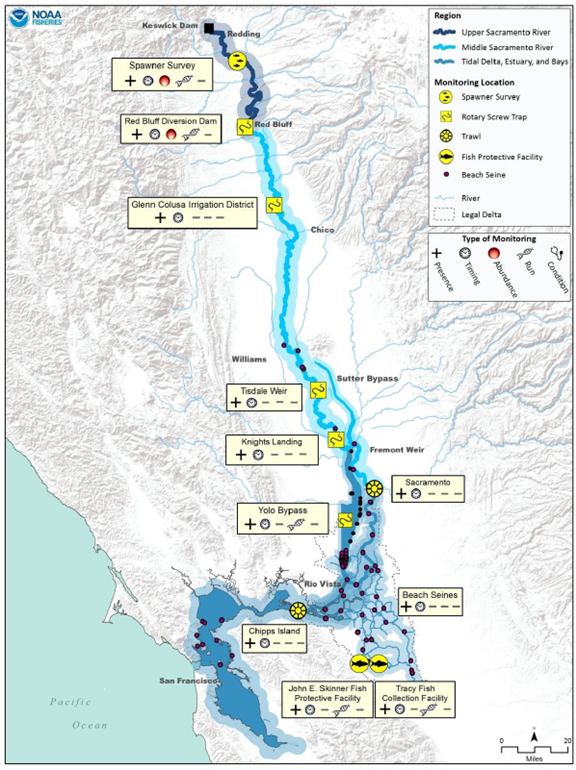
\includegraphics{figures/map_sac_river_delta_bay.png}
\caption{``distribution map''}
\end{figure}

\hypertarget{conceptual-model}{%
\section{Conceptual Model}\label{conceptual-model}}

Metrics selected in this report are based on a conceptual model developed by Windell et al.~(2017).

\begin{figure}
\centering
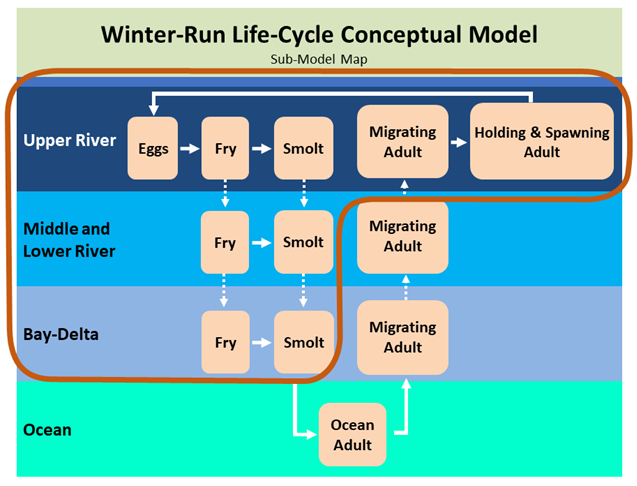
\includegraphics{figures/WRCM.png}
\caption{``conceptual model''}
\end{figure}

\hypertarget{references}{%
\section{References}\label{references}}

\begin{itemize}
\tightlist
\item
  \url{https://wildlife.ca.gov/Conservation/Fishes/Chinook-Salmon/Winter-run}
\item
  Moyle P.B. 2002. Inland Fishes of California, University of California Press.
\item
  National Marine Fisheries Service (NMFS). 2014. Recovery Plan for Evolutionarily Significant Units of Sacramento River Winter-run Chinook Salmon and Central Valley Spring-run Chinook Salmon and the Distinct population Segment of California Central Valley Steelhead. California Central Valley Area Office, July 2014.
\item
  Windell, S., P.L. Brandes, J.L. Conrad, J.W. Ferguson, P.A.L. Goertler, B.N. Harvey, J. Heublein, J.A. Israel, D.W. Kratville, J.E. Kirsch, R.W. Perry, J. Pisciotto, W.R. Poytress, K. Reece, B.G. Swart, and R.C. Johnson, 2017. Scientific Framework for Assessing Factors Influencing Endangered Sacramento River Winter­Run Chinook Salmon (Oncorhynchus tshawytscha) Across the Life Cycle. NOAA Technical Memorandum NMFS. NOAA-TM-NMFS-SWFSC-586. August 2017. Available at: \url{https://watershed.ucdavis.edu/files/biblio/NOAA-TM-NMFS-SWFSC-586_Final.pdf}
\end{itemize}

\hypertarget{adults}{%
\chapter{Adults}\label{adults}}

This section describes environmental attributes associated with and responses during the adult life stage (ocean harvest, migration, spawning)

\hypertarget{habitat-attributes}{%
\section{Habitat Attributes}\label{habitat-attributes}}

\begin{enumerate}
\def\labelenumi{\arabic{enumi}.}
\item
  Hatchery Influence (Proportion of hatchery return)
\item
  Spawning Habitat Capacity (SIT model)
\end{enumerate}

\hypertarget{wq}{%
\section{Environmental Drivers}\label{wq}}

2021 was a Critical water year type and 2020 was a Dry water year type.

\hypertarget{storage-and-flow}{%
\subsection{Storage and Flow}\label{storage-and-flow}}

\hypertarget{shasta-storage}{%
\subsubsection{Shasta Storage}\label{shasta-storage}}

Flows in the Sacramento River are dependent on Shasta storage. Adult WR Chinook Salmon rely on flows for migration cues.

\label{fig:SHAstor-fig}Daily Shasta Dam Storage (SHA) in 2021 and over the 10-year average.

\hypertarget{flow-conditions-on-the-upper-sacramento-river}{%
\subsubsection{Flow Conditions on the Upper Sacramento River}\label{flow-conditions-on-the-upper-sacramento-river}}

\label{fig:KWKBNDflow-fig}Daily Flows (cfs) at Sacramento Rier at Keswick (KWK) and Sacramento River at Bend Bridge (BND) in 2021 and over the 10-year average

\begin{table}
\centering
\caption{Mean, Maximum, Minimum Monthly Flows (cfs) at Sacramento River at Keswick (KWK) and Sacramento River at Bend Bridge (BND)  in 2021}
\centering
\begin{tabular}[t]{rllrrr}
\hline
Year & Month & Station & Mean & Min & Max\\
\hline
2021 & January & BND & 6982.1 & 4220 & 12300\\
\hline
2021 & February & BND & 7358.0 & 4560 & 13500\\
\hline
2021 & March & BND & 7048.8 & 4540 & 10100\\
\hline
2021 & April & BND & 6666.7 & 4590 & 8920\\
\hline
2021 & May & BND & 8858.0 & 7170 & 10800\\
\hline
2021 & June & BND & 8328.5 & 7180 & 9330\\
\hline
2021 & July & BND & 9642.1 & 9030 & 10600\\
\hline
2021 & August & BND & 8334.2 & 6840 & 9670\\
\hline
2021 & September & BND & 7072.0 & 6840 & 7300\\
\hline
2021 & October & BND & 13618.0 & 6220 & 36800\\
\hline
2021 & November & BND & 8279.9 & 4260 & 17700\\
\hline
2021 & December & BND & 10327.5 & 4220 & 26600\\
\hline
2021 & January & KWK & 3217.4 & 2970 & 3700\\
\hline
2021 & February & KWK & 3157.9 & 2900 & 3520\\
\hline
2021 & March & KWK & 3405.0 & 3170 & 3640\\
\hline
2021 & April & KWK & 5682.5 & 3280 & 8050\\
\hline
2021 & May & KWK & 8369.6 & 6800 & 9870\\
\hline
2021 & June & KWK & 7882.3 & 6570 & 9390\\
\hline
2021 & July & KWK & 9510.2 & 8740 & 10800\\
\hline
2021 & August & KWK & 8102.0 & 6610 & 9500\\
\hline
2021 & September & KWK & 6899.8 & 5310 & 8500\\
\hline
2021 & October & KWK & 6160.1 & 5120 & 7330\\
\hline
2021 & November & KWK & 4027.1 & 3070 & 5080\\
\hline
2021 & December & KWK & 3431.0 & 3040 & 3970\\
\hline
\end{tabular}
\end{table}

\textbf{Summary}

\begin{itemize}
\tightlist
\item
  In 2021, storage was consistently below the 10-year average (Figure \ref{fig:SHAstor-fig}), with peak storage at \textbf{2.4} TAF in \textbf{4}.
\item
  \textbf{Keswick:} Peak flows were \textbf{\ensuremath{1.08\times 10^{4}}} cfs and occurred in \textbf{7}. The highest mean flows were \textbf{9510.2} cfs and occurred in \textbf{7}.
\item
  \textbf{Bend Bridge:} Peak flows were \textbf{\ensuremath{3.68\times 10^{4}}} cfs and occurred in \textbf{10}. The highest mean flows were \textbf{\ensuremath{1.3618\times 10^{4}}} cfs and occurred in \textbf{10}.
\end{itemize}

\hypertarget{water-temperature}{%
\subsection{Water Temperature}\label{water-temperature}}

\hypertarget{temp-thresholds}{%
\subsubsection{Temperature Threshold Analysis}\label{temp-thresholds}}

The temperature compliance point (location of compliance to daily average temperature (DAT) of ≤56°F) varies annually based on USBR's Temperature Management Plan.

\textbf{Summary}

\begin{itemize}
\tightlist
\item
  The compliance point at X was met X percent of days (\ref{fig:tempthresholdanalysis-fig}).
\end{itemize}

\hypertarget{water-temperature-at-balls-ferry-bridge-and-clear-creek}{%
\subsubsection{Water Temperature at Balls Ferry Bridge and Clear Creek}\label{water-temperature-at-balls-ferry-bridge-and-clear-creek}}

\label{fig:historicalwtemp-fig}Daily Water Temperature at Sacramento River at Clear Creek (CCR) and Sacramento River at Balls Ferry Bridge (BSF) in 2021 and over the 10-year average

\begin{table}
\centering
\caption{Mean, Maximum, Minimum Monthly Water Temperature (°F) at Sacramento River at Balls Ferry Bridge (BSF) and Sacramento River upstream from Confluence with Clear Creek (CCR) in 2021}
\centering
\begin{tabular}[t]{rllrrr}
\hline
Year & Month & Station & Mean & Min & Max\\
\hline
2021 & January & BSF & 48.6 & 44.2 & 52.4\\
\hline
2021 & February & BSF & 49.2 & 46.2 & 52.1\\
\hline
2021 & March & BSF & 51.7 & 47.2 & 56.2\\
\hline
2021 & April & BSF & 56.6 & 51.3 & 62.4\\
\hline
2021 & May & BSF & 59.9 & 54.8 & 65.4\\
\hline
2021 & June & BSF & 58.2 & 53.8 & 62.7\\
\hline
2021 & July & BSF & 57.6 & 54.6 & 60.7\\
\hline
2021 & August & BSF & 57.8 & 54.5 & 66.9\\
\hline
2021 & September & BSF & 59.0 & 56.2 & 61.9\\
\hline
2021 & October & BSF & 59.3 & 56.9 & 61.7\\
\hline
2021 & November & BSF & 56.4 & 52.3 & 60.5\\
\hline
2021 & December & BSF & 50.7 & 46.0 & 55.4\\
\hline
2021 & January & CCR & 50.0 & 46.5 & 53.2\\
\hline
2021 & February & CCR & 50.1 & 47.8 & 52.4\\
\hline
2021 & March & CCR & 51.6 & 47.9 & 55.4\\
\hline
2021 & April & CCR & 55.3 & 50.1 & 61.0\\
\hline
2021 & May & CCR & 59.4 & 54.7 & 64.5\\
\hline
2021 & June & CCR & 56.3 & 53.0 & 59.6\\
\hline
2021 & July & CCR & 56.0 & 53.9 & 58.1\\
\hline
2021 & August & CCR & 57.1 & 54.3 & 60.1\\
\hline
2021 & September & CCR & 58.6 & 55.9 & 61.4\\
\hline
2021 & October & CCR & 59.7 & 57.3 & 62.1\\
\hline
2021 & November & CCR & 57.0 & 53.4 & 61.0\\
\hline
2021 & December & CCR & 52.4 & 48.1 & 56.7\\
\hline
\end{tabular}
\end{table}

\textbf{Summary}

\begin{itemize}
\tightlist
\item
  Water temperatures were warmer than average and warmer than 56°F in 2021 (Figure \ref{fig:historicalwtemp-fig}).
\item
  \textbf{Balls Ferry:} Maximum water temperature was \textbf{66.9} degrees F and occurred in \textbf{8}. The highest mean water temperature was \textbf{59.9} degrees F and occurred in \textbf{5}.
\item
  \textbf{Clear Creek:} Maximum water temperature was \textbf{64.5} degrees F and occurred in \textbf{5}. The highest mean water temperature was \textbf{59.7} degrees F and occurred in \textbf{10}.
\end{itemize}

\hypertarget{dissolved-oxygen-conditions-at-keswick-dam-and-clear-creek}{%
\subsection{Dissolved Oxygen Conditions at Keswick Dam and Clear Creek}\label{dissolved-oxygen-conditions-at-keswick-dam-and-clear-creek}}

\label{fig:KWKCCRDO-fig}Daily Dissolved Oxygen (mg/L) at Sacramento River at Keswick Dam (KWK) and Sacramento River upstream from Confluence with Clear Creek (CCR).

\begin{table}
\centering
\caption{Mean, Maximum, Minimum Monthly Dissolved Oxygen (mg/L) at Sacramento River at Keswick (KWK) and Sacramento River upstream from Confluence with Clear Creek (CCR)  in 2021}
\centering
\begin{tabular}[t]{rllrrr}
\hline
Year & Month & Station & Mean & Min & Max\\
\hline
2021 & January & CCR & 13.0 & 11.2 & 14.8\\
\hline
2021 & February & CCR & 13.5 & 8.8 & 15.9\\
\hline
2021 & March & CCR & 13.4 & 11.5 & 15.4\\
\hline
2021 & April & CCR & 12.9 & 11.1 & 14.8\\
\hline
2021 & May & CCR & 12.7 & 10.4 & 14.9\\
\hline
2021 & June & CCR & 12.9 & 10.6 & 15.2\\
\hline
2021 & July & CCR & 12.8 & 10.3 & 15.3\\
\hline
2021 & August & CCR & 11.6 & 10.0 & 13.1\\
\hline
2021 & September & CCR & 11.4 & 9.1 & 13.8\\
\hline
2021 & October & CCR & 10.8 & 8.7 & 12.8\\
\hline
2021 & November & CCR & 8.3 & 6.6 & 10.1\\
\hline
2021 & December & CCR & 13.3 & 8.3 & 17.3\\
\hline
2021 & January & KWK & 13.1 & 12.1 & 14.0\\
\hline
2021 & February & KWK & 13.6 & 12.6 & 14.6\\
\hline
2021 & March & KWK & 13.3 & 12.3 & 14.4\\
\hline
2021 & April & KWK & 10.8 & 8.2 & 14.1\\
\hline
2021 & May & KWK & 8.9 & 7.4 & 10.7\\
\hline
2021 & June & KWK & 9.6 & 8.5 & 10.7\\
\hline
2021 & July & KWK & 7.2 & 2.5 & 11.0\\
\hline
2021 & August & KWK & 11.1 & 10.0 & 12.1\\
\hline
2021 & September & KWK & 12.7 & 8.6 & 15.8\\
\hline
2021 & October & KWK & 8.7 & 7.8 & 9.4\\
\hline
2021 & November & KWK & 10.0 & 8.4 & 11.6\\
\hline
2021 & December & KWK & 12.7 & 11.4 & 14.0\\
\hline
\end{tabular}
\end{table}

\textbf{Summary}

\begin{itemize}
\tightlist
\item
  \textbf{Keswick:} Minimum dissolved oxygen was \textbf{2.5} mg/L and occurred in \textbf{7}. The lowest mean dissolved oxygen was \textbf{7.2} mg/L and occurred in \textbf{7}.
\item
  \textbf{Clear Creek:} Minimum dissolved oxygen was \textbf{6.6} mg/L and occurred in \textbf{11}. The lowest mean dissolved oxygen was \textbf{8.3} mg/L and occurred in \textbf{11}.
\end{itemize}

\hypertarget{biological-response}{%
\section{Biological Response}\label{biological-response}}

\textbf{Data Sources}

\begin{itemize}
\tightlist
\item
  Sex and age class distribution, \% spawned, spawn origin, spawn timing: Carcass Survey Data (link)
\item
  Pre-spawn mortality: JPE Letters and USFWS Reports (link)
\item
  Redd abundance and distribution: Aerial redd data
\item
  Carcass abundance and distribution: Carcass data
\end{itemize}

\hypertarget{adult-survival}{%
\subsection{Adult Survival}\label{adult-survival}}

In-river escapement decreased after the construction of the Red Bluff Diversion Dam (RBDD) in the 1960s.

\begin{itemize}
\tightlist
\item
  Sacramento River system-wide total adult escapement: \ensuremath{1.0165\times 10^{4}}

  \begin{itemize}
  \tightlist
  \item
    10-year average: 4416
  \item
    20-year average: 5612
  \end{itemize}
\item
  Total mainstem in-river spawner estimate (Killam): 9998, 90\% Confidence Interval: {[}{]}

  \begin{itemize}
  \tightlist
  \item
    10-year average: 4302
  \item
    20-year average: 5555
  \end{itemize}
\item
  Mainstem natural-origin spawners (Killam): 64.5 \%
\item
  Mainstem hatchery-origin spawners (Killam): 35.5 \%

  \begin{itemize}
  \tightlist
  \item
    10-year average:
  \end{itemize}
\item
  Fish to hatchery broodstock (Killam):

  \begin{itemize}
  \tightlist
  \item
    In-river mainstem transferred to Livingston Stone National Fish Hatchery (LSNFH): 298
  \item
    In-river mainstem transferred to Coleman National Fish Hatchery (CNFH): 58
  \end{itemize}
\item
  Tributary in-river spawners (Killam):

  \begin{itemize}
  \tightlist
  \item
    Battle Creek:167
  \item
    Clear Creek: 0
  \end{itemize}
\end{itemize}

\begin{figure}
\centering
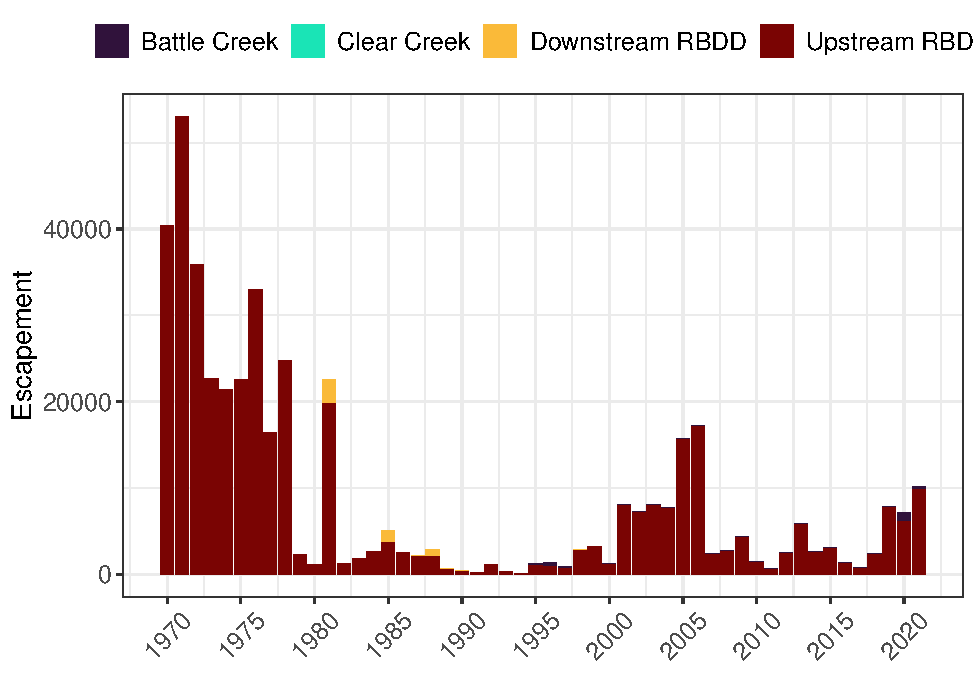
\includegraphics{_main_files/figure-latex/unnamed-chunk-9-1.pdf}
\caption{\label{fig:unnamed-chunk-9}Estimated Total Mainstem In-River Spawners in 2021by reach. Data from SacPAS.}
\end{figure}

Placeholder for Annual Replacement Rate Plot

\begin{figure}
\centering
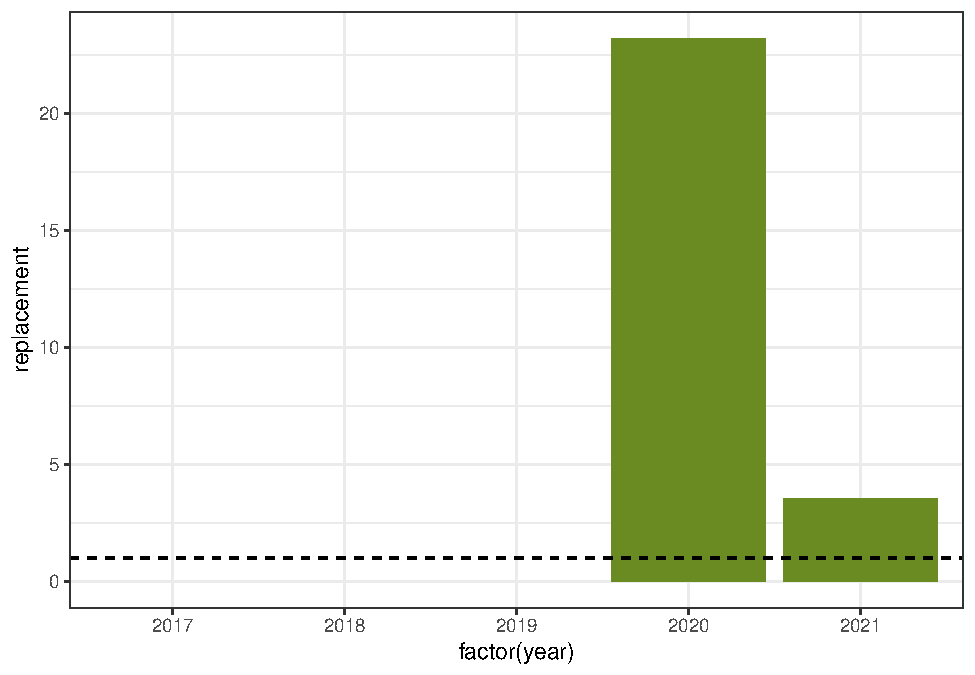
\includegraphics{_main_files/figure-latex/cohortreplacement-fig-1.pdf}
\caption{\label{fig:cohortreplacement-fig}Cohort Replacement Rate. Current year spawners are divided by number of spawners from 3 years ago. Horizontal line is at 1.0.}
\end{figure}

\begin{table}
\centering
\caption{Escapement by Reach}
\centering
\begin{tabular}[t]{rrrrrr}
\hline
Year & Downstream RBDD & Upstream RBDD & Clear Creek & Battle Creek & Total\\
\hline
2021 & 0 & 9998 & 0 & 167 & 10165\\
\hline
2020 & 0 & 6199 & 0 & 942 & 7141\\
\hline
2019 & 0 & 7853 & 0 & 21 & 7874\\
\hline
2018 & 0 & 2458 & 0 & 1 & 2459\\
\hline
2017 & 0 & 797 & 2 & 0 & 799\\
\hline
2016 & 0 & 1411 & 1 & 0 & 1412\\
\hline
2015 & 0 & 3182 & NA & 0 & 3182\\
\hline
2014 & 0 & 2627 & NA & 0 & 2627\\
\hline
2013 & 0 & 5922 & NA & 0 & 5922\\
\hline
2012 & 0 & 2578 & NA & 0 & 2578\\
\hline
2011 & 0 & 738 & NA & 1 & 739\\
\hline
2010 & 0 & 1533 & NA & 0 & 1533\\
\hline
2009 & 0 & 4416 & NA & 0 & 4416\\
\hline
2008 & 0 & 2725 & NA & 0 & 2725\\
\hline
2007 & 0 & 2487 & NA & 0 & 2487\\
\hline
2006 & 48 & 17149 & NA & 6 & 17203\\
\hline
2005 & 0 & 15730 & NA & 0 & 15730\\
\hline
2004 & 0 & 7784 & NA & 0 & 7784\\
\hline
2003 & 28 & 8105 & NA & 0 & 8133\\
\hline
2002 & 12 & 7325 & NA & 0 & 7337\\
\hline
2001 & 35 & 8085 & NA & 0 & 8120\\
\hline
2000 & 0 & 1261 & NA & 2 & 1263\\
\hline
1999 & 0 & 3264 & NA & NA & 3264\\
\hline
1998 & 62 & 2831 & NA & NA & 2893\\
\hline
1997 & 0 & 836 & NA & 44 & 880\\
\hline
1996 & 0 & 1012 & NA & 325 & 1337\\
\hline
1995 & 7 & 1159 & NA & 88 & 1254\\
\hline
1994 & 0 & 144 & NA & NA & 144\\
\hline
1993 & 9 & 369 & NA & NA & 378\\
\hline
1992 & 44 & 1159 & NA & NA & 1203\\
\hline
1991 & 0 & 177 & NA & NA & 177\\
\hline
1990 & 28 & 384 & NA & NA & 412\\
\hline
1989 & 14 & 635 & NA & NA & 649\\
\hline
1988 & 728 & 2129 & NA & NA & 2857\\
\hline
1987 & 97 & 2068 & NA & NA & 2165\\
\hline
1986 & NA & 2566 & NA & NA & 2566\\
\hline
1985 & 1445 & 3686 & NA & NA & 5131\\
\hline
1984 & NA & 2662 & NA & NA & 2662\\
\hline
1983 & NA & 1827 & NA & NA & 1827\\
\hline
1982 & 39 & 1233 & NA & NA & 1272\\
\hline
1981 & 2756 & 19795 & NA & NA & 22551\\
\hline
1980 & NA & 1142 & NA & NA & 1142\\
\hline
1979 & NA & 2339 & NA & NA & 2339\\
\hline
1978 & NA & 24735 & NA & NA & 24735\\
\hline
1977 & NA & 16470 & NA & NA & 16470\\
\hline
1976 & NA & 33029 & NA & NA & 33029\\
\hline
1975 & NA & 22579 & NA & NA & 22579\\
\hline
1974 & NA & 21389 & NA & NA & 21389\\
\hline
1973 & NA & 22651 & NA & NA & 22651\\
\hline
1972 & NA & 35929 & NA & NA & 35929\\
\hline
1971 & NA & 53089 & NA & NA & 53089\\
\hline
1970 & NA & 40409 & NA & NA & 40409\\
\hline
\end{tabular}
\end{table}

\hypertarget{fish-condition-and-age-class}{%
\subsection{Fish Condition and Age Class}\label{fish-condition-and-age-class}}

\begin{itemize}
\tightlist
\item
  Pre-spawn mortality: 4.8\%

  \begin{itemize}
  \tightlist
  \item
    10-year average:
  \item
    10-year maximum:
  \item
    20-year average:
  \item
    20-year maximum:
  \end{itemize}
\item
  Fecundity: 5312 eggs per female

  \begin{itemize}
  \tightlist
  \item
    10-year average: 4812 eggs per female
  \item
    20-year average: 4998 eggs per female (only goes to 2005)
  \end{itemize}
\item
  Age classes based on size:

  \begin{itemize}
  \tightlist
  \item
    Jacks and Jills = Age-2 fish
  \item
    Percent Adult Female (\textgreater=610 millimeters {[}mm{]}): 73.5\%
  \item
    Percent Jills (\textless610 mm): 0.9\%
  \item
    Percent Adult Male (\textgreater=680 mm): 23.3\%
  \item
    Percent Jacks (\textless680 mm): 1.9\%
  \end{itemize}
\end{itemize}

\begin{table}
\centering
\caption{Carcass Data Summary. Fork length cutoffs are 610 mm for Females and 680 mm for Males based on Killam 2021}
\centering
\begin{tabular}[t]{lrrrrr}
\hline
Age Class & Count & Mean FL (mm) & SD & Min FL (mm) & Max FL (mm)\\
\hline
Female Adult & 2504 & 744 & 46 & 610 & 911\\
\hline
Jack & 65 & 581 & 53 & 469 & 679\\
\hline
Jill & 30 & 572 & 42 & 412 & 609\\
\hline
Male Adult & 794 & 854 & 61 & 680 & 1065\\
\hline
\end{tabular}
\end{table}

\begin{figure}
\centering
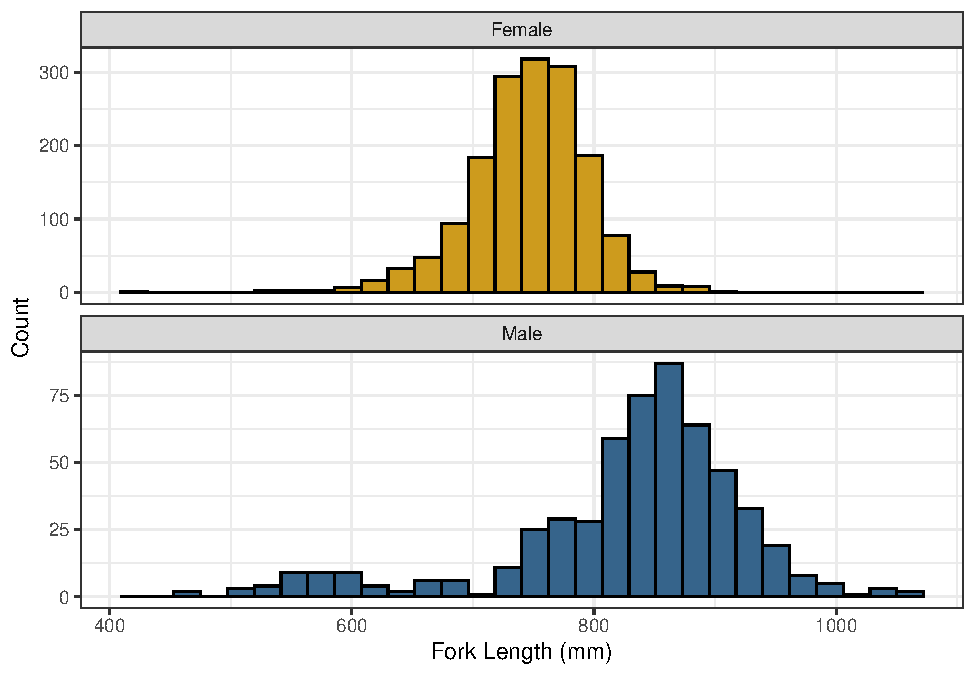
\includegraphics{_main_files/figure-latex/carcassFL-fig-1.pdf}
\caption{\label{fig:carcassFL-fig}Carcass Data Fork Length Distribution. Plots are separated by Sex.}
\end{figure}

\hypertarget{migration-and-spawn-timing}{%
\subsection{Migration and Spawn Timing}\label{migration-and-spawn-timing}}

\hypertarget{spawn-timing}{%
\subsubsection{Spawn Timing}\label{spawn-timing}}

\begin{figure}
\centering
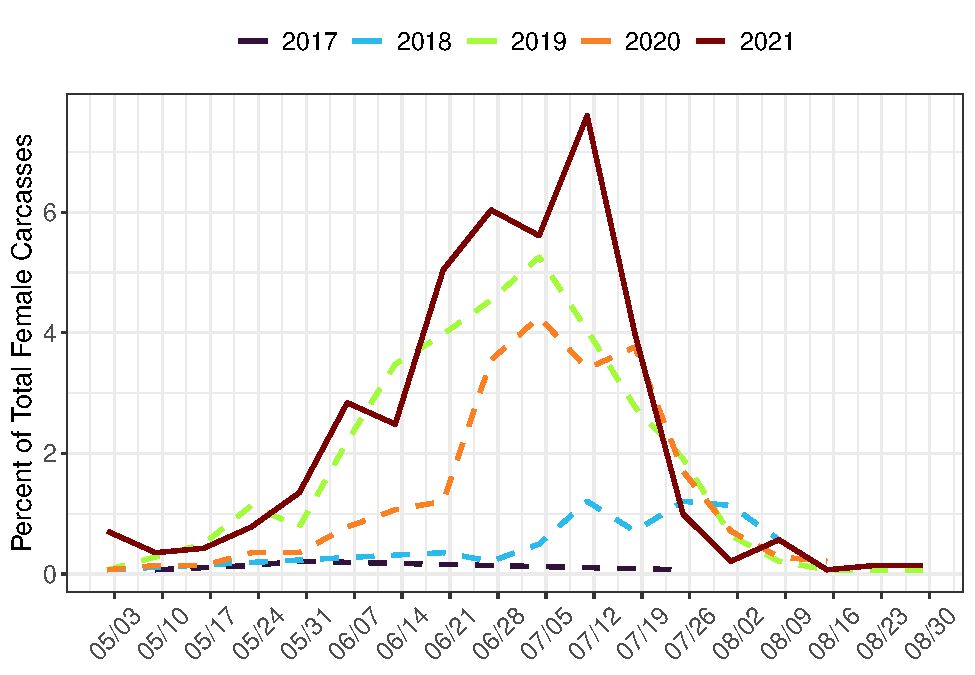
\includegraphics{_main_files/figure-latex/spawntiming-fig-1.pdf}
\caption{\label{fig:spawntiming-fig}Spawn Timing, 2017 through 2021}
\end{figure}

Add 10-year and 20-year average to this plot.

\begin{figure}
\centering
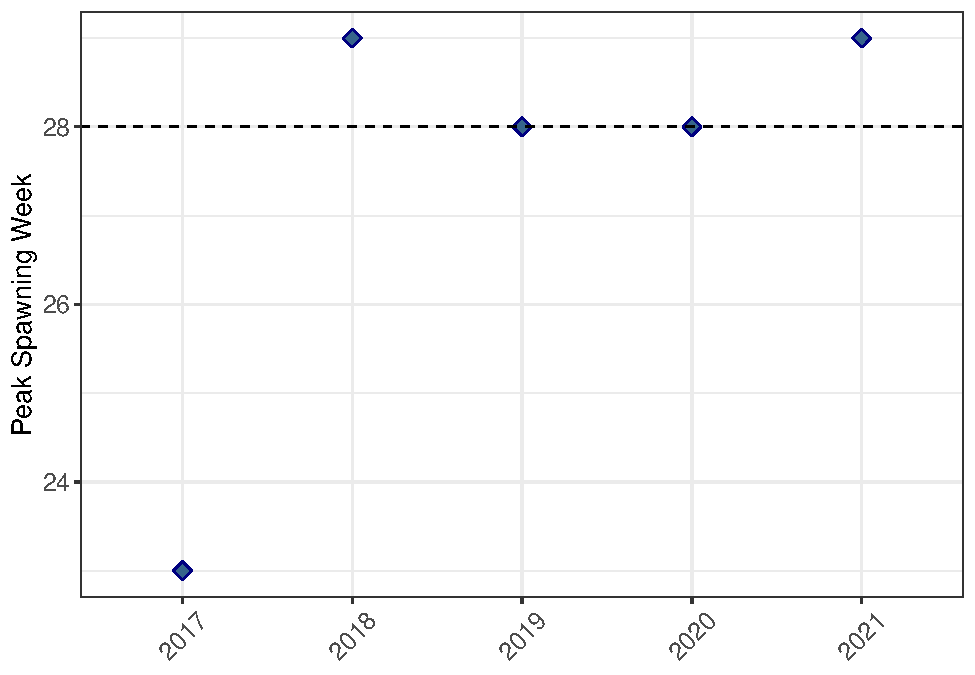
\includegraphics{_main_files/figure-latex/spawnweek-fig-1.pdf}
\caption{\label{fig:spawnweek-fig}Peak Spawning Week from 2000 to 2021}
\end{figure}

Expand data to include more years (should have 10-year median and 20-year median)

\hypertarget{carcass-and-redd-abundance-and-distribution}{%
\subsection{Carcass and Redd Abundance and Distribution}\label{carcass-and-redd-abundance-and-distribution}}

\hypertarget{redd-abundance}{%
\subsubsection{Redd Abundance}\label{redd-abundance}}

\begin{table}
\centering
\caption{Redd Abundance by Section in 2021}
\centering
\begin{tabular}[t]{llrrr}
\hline
Section & Section Name & Count & Percent & Average\\
\hline
1 & A.C.I.D. Dam to Keswick Dam & NA & NA & 8.00\%\\
\hline
2 & Hwy 44 Brg to A.C.I.D Dam & 484 & 100.00\% & 85.00\%\\
\hline
3 & Clear Crk. Powerlines to Hwy 44 Brg & NA & NA & 10.00\%\\
\hline
4 & Balls Ferry Brg to Clear Crk Powerlines & NA & NA & 0.00\%\\
\hline
7 & Bend Brg to Jellys Brg & NA & NA & 1.00\%\\
\hline
\end{tabular}
\end{table}

\hypertarget{carcass-abundance}{%
\subsubsection{Carcass Abundance}\label{carcass-abundance}}

\begin{table}
\centering
\caption{Carcass Abundance by Section in 2021}
\centering
\begin{tabular}[t]{llrrr}
\hline
Section Name & Section & Count & Percent & Average\\
\hline
Keswick to ACID (RM 302-298) & 1 & 320 & 37.00\% & 18.00\%\\
\hline
ACID to Hwy 44 Bridge (RM 298-296) & 2 & 190 & 22.00\% & 22.00\%\\
\hline
Hwy 44 Bridge to Clear Creek PLs (RM 296-288) & 3 & 270 & 31.00\% & 38.00\%\\
\hline
Clear Creek PLs to Balls Ferry Bridge (RM 288-276) & 4 & 89 & 10.00\% & 21.00\%\\
\hline
\end{tabular}
\end{table}

\label{fig:redds-fig}Redd Counts by Year. Dashed line indicates average from 2013 to 2021

It would be nice to include here a map of each reach

\hypertarget{redd-distribution}{%
\subsubsection{Redd Distribution}\label{redd-distribution}}

\begin{figure}
\centering
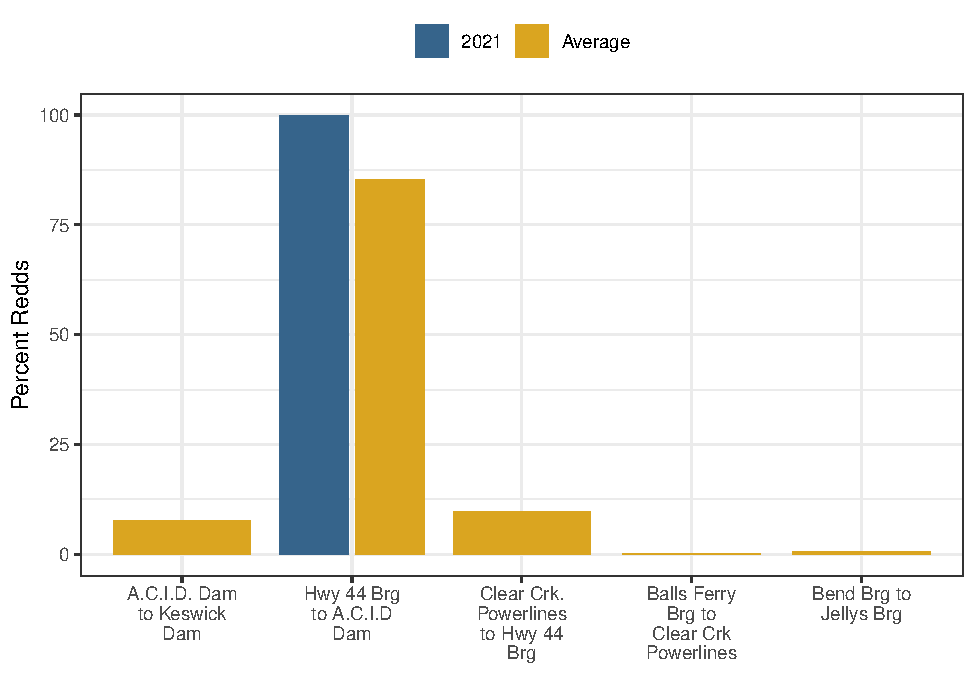
\includegraphics{_main_files/figure-latex/redddistrib-fig-1.pdf}
\caption{\label{fig:redddistrib-fig}Distribution of Winter Run Redds in 2021 and Average between 2013 and 2021}
\end{figure}

\hypertarget{carcass-distribution}{%
\subsubsection{Carcass Distribution}\label{carcass-distribution}}

\begin{figure}
\centering
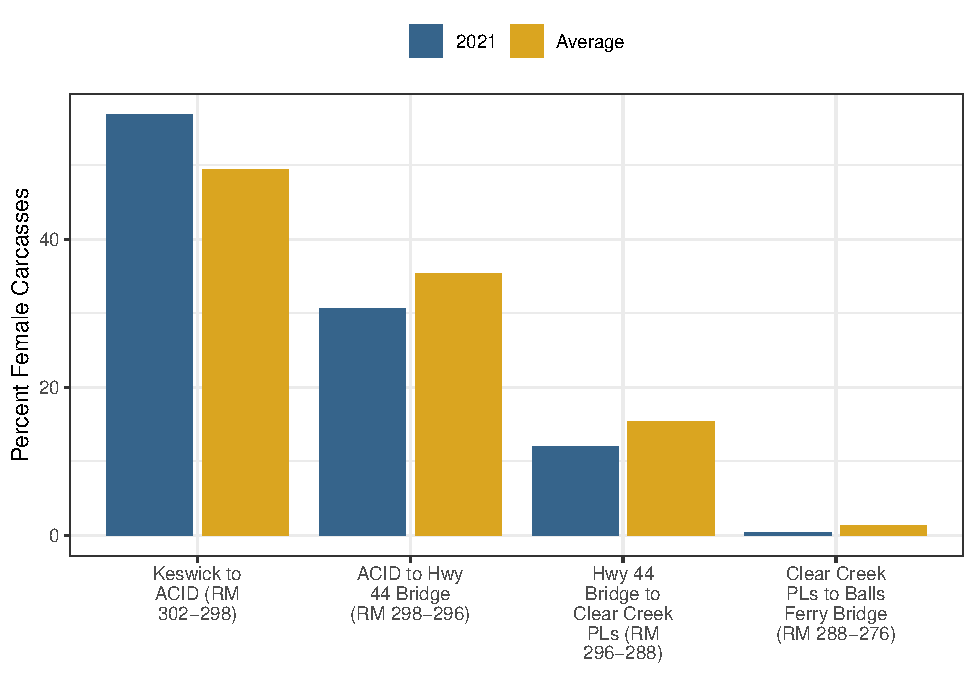
\includegraphics{_main_files/figure-latex/carcassdistrib-fig-1.pdf}
\caption{\label{fig:carcassdistrib-fig}Female Carcass Distribution for 2021 and Average from 2017 to 2021}
\end{figure}

\hypertarget{egg-to-fry-emergence}{%
\chapter{Egg to Fry Emergence}\label{egg-to-fry-emergence}}

This section describes environmental attributes associated with and responses during the egg-to-fry life stage.

\hypertarget{environmental-drivers}{%
\section{Environmental Drivers}\label{environmental-drivers}}

\hypertarget{storage-and-flow-1}{%
\subsection{Storage and Flow}\label{storage-and-flow-1}}

\hypertarget{shasta-storage-1}{%
\subsubsection{Shasta Storage}\label{shasta-storage-1}}

\begin{itemize}
\tightlist
\item
  See \ref{shasta-storage} for summary of storage conditions.
\end{itemize}

\hypertarget{flow-conditions-on-the-upper-sacramento-river-1}{%
\subsubsection{Flow Conditions on the Upper Sacramento River}\label{flow-conditions-on-the-upper-sacramento-river-1}}

\begin{table}
\centering
\caption{Mean, Maximum, Minimum Monthly Flows (cfs) at Sacramento River at Keswick (KWK) and Sacramento River at Bend Bridge (BND) between May and November 2021}
\centering
\begin{tabular}[t]{rllrrr}
\hline
Year & Station & Month & Mean & Min & Max\\
\hline
2021 & KWK & May & 8369.6 & 6800 & 9870\\
\hline
2021 & KWK & June & 7882.3 & 6570 & 9390\\
\hline
2021 & KWK & July & 9510.2 & 8740 & 10800\\
\hline
2021 & KWK & August & 8102.0 & 6610 & 9500\\
\hline
2021 & KWK & September & 6899.8 & 5310 & 8500\\
\hline
2021 & KWK & October & 6160.1 & 5120 & 7330\\
\hline
2021 & KWK & November & 4027.1 & 3070 & 5080\\
\hline
2021 & BND & May & 8858.0 & 7170 & 10800\\
\hline
2021 & BND & June & 8328.5 & 7180 & 9330\\
\hline
2021 & BND & July & 9642.1 & 9030 & 10600\\
\hline
2021 & BND & August & 8334.2 & 6840 & 9670\\
\hline
2021 & BND & September & 7072.0 & 6840 & 7300\\
\hline
2021 & BND & October & 13618.0 & 6220 & 36800\\
\hline
2021 & BND & November & 8279.9 & 4260 & 17700\\
\hline
\end{tabular}
\end{table}

\begin{itemize}
\tightlist
\item
  \textbf{Keswick:} Peak flows were \textbf{\ensuremath{1.08\times 10^{4}}} cfs and occurred in \textbf{7}. The highest mean flows were \textbf{9510.2} cfs and occurred in \textbf{7}.
\item
  \textbf{Bend Bridge:} Peak flows were \textbf{\ensuremath{3.68\times 10^{4}}} cfs and occurred in \textbf{10}. The highest mean flows were \textbf{\ensuremath{1.3618\times 10^{4}}} cfs and occurred in \textbf{10}.
\end{itemize}

\hypertarget{water-temperature-on-the-upper-sacramento-river}{%
\subsection{Water Temperature on the Upper Sacramento River}\label{water-temperature-on-the-upper-sacramento-river}}

\begin{itemize}
\tightlist
\item
  See \ref{temp-thresholds} for discussion around temperature threshold analysis.
\end{itemize}

\hypertarget{dissolved-oxygen-conditions-on-the-upper-sacramento-river}{%
\subsection{Dissolved Oxygen Conditions on the Upper Sacramento River}\label{dissolved-oxygen-conditions-on-the-upper-sacramento-river}}

\begin{table}
\centering
\caption{Mean, Maximum, Minimum Monthly Dissolved Oxygen (mg/L) at Sacramento River at Keswick (KWK) and Sacramento River upstream from Confluence with Clear Creek (CCR) between May and November 2021}
\centering
\begin{tabular}[t]{rllrrr}
\hline
Year & Station & Month & Mean & Min & Max\\
\hline
2021 & KWK & May & 8.9 & 7.4 & 10.7\\
\hline
2021 & KWK & June & 9.6 & 8.5 & 10.7\\
\hline
2021 & KWK & July & 7.2 & 2.5 & 11.0\\
\hline
2021 & KWK & August & 11.1 & 10.0 & 12.1\\
\hline
2021 & KWK & September & 12.7 & 8.6 & 15.8\\
\hline
2021 & KWK & October & 8.7 & 7.8 & 9.4\\
\hline
2021 & KWK & November & 10.0 & 8.4 & 11.6\\
\hline
2021 & CCR & May & 12.7 & 10.4 & 14.9\\
\hline
2021 & CCR & June & 12.9 & 10.6 & 15.2\\
\hline
2021 & CCR & July & 12.8 & 10.3 & 15.3\\
\hline
2021 & CCR & August & 11.6 & 10.0 & 13.1\\
\hline
2021 & CCR & September & 11.4 & 9.1 & 13.8\\
\hline
2021 & CCR & October & 10.8 & 8.7 & 12.8\\
\hline
2021 & CCR & November & 8.3 & 6.6 & 10.1\\
\hline
\end{tabular}
\end{table}

\textbf{Summary}

\begin{itemize}
\tightlist
\item
  \textbf{Keswick:} Minimum dissolved oxygen was \textbf{2.5} mg/L and occurred in \textbf{7}. The lowest mean dissolved oxygen was \textbf{7.2} mg/L and occurred in \textbf{7}.
\item
  \textbf{Clear Creek:} Minimum dissolved oxygen was \textbf{6.6} mg/L and occurred in \textbf{11}. The lowest mean dissolved oxygen was \textbf{8.3} mg/L and occurred in \textbf{11}.
\end{itemize}

\hypertarget{air-temperature}{%
\subsection{Air Temperature}\label{air-temperature}}

\label{fig:KRDDatemp-fig}Daily Air Temperature (deg F) at Redding Municipal Airport from May 2021 through November 2021 and maximum and minimum temperatures since 2003

\hypertarget{biological-response-1}{%
\section{Biological Response}\label{biological-response-1}}

\hypertarget{egg-to-fry-survival}{%
\subsection{Egg to Fry Survival}\label{egg-to-fry-survival}}

\textbf{Egg-to-Fry Metrics}

\begin{itemize}
\tightlist
\item
  \textbf{Total potential eggs:} 31,128,320 eggs

  \begin{itemize}
  \tightlist
  \item
    \textbf{10-year average:} 12,855,143 eggs
  \item
    \textbf{20-year average:} 16,534,741 eggs
  \end{itemize}
\item
  \textbf{Fry-equivalents at RBDD (JPE Letter):} .

  \begin{itemize}
  \tightlist
  \item
    \textbf{10-year average:} 583,767 including 2011, 2014-2017, 2021
  \end{itemize}
\item
  \textbf{Egg to Fry Survival (ETF Survival):} ETF Survival in 2021 was below the average ETF between 2002 and 2021 at 2.5\% (Figure \ref{fig:ETFSurv-fig}).

  \begin{itemize}
  \tightlist
  \item
    The average ETF from 1970 to 2021 was 22.335\%
  \end{itemize}
\end{itemize}

\hypertarget{sacpas-fish-model}{%
\subsubsection{SacPAS Fish Model}\label{sacpas-fish-model}}

\begin{itemize}
\tightlist
\item
  Redds exposed to Tcritical = 11.82°C (53.28°F) are shown in Figure X.

  \begin{itemize}
  \tightlist
  \item
    Pre-hatching exposure:
  \item
    Pre-emergence exposure:
  \end{itemize}
\item
  Estimated total egg-to-fry emergence survival:

  \begin{itemize}
  \tightlist
  \item
    Temperature-dependent survival:
  \end{itemize}
\item
  TDM

  \begin{itemize}
  \tightlist
  \item
    Spawner density-based survival:
    ‒ Background survival:
    ‒ Dewater-based survival:
    ‒ Survival by reach is shown in Table X
  \end{itemize}
\end{itemize}

Table of Survival by Reach (Fish Model)

\begin{figure}
\centering
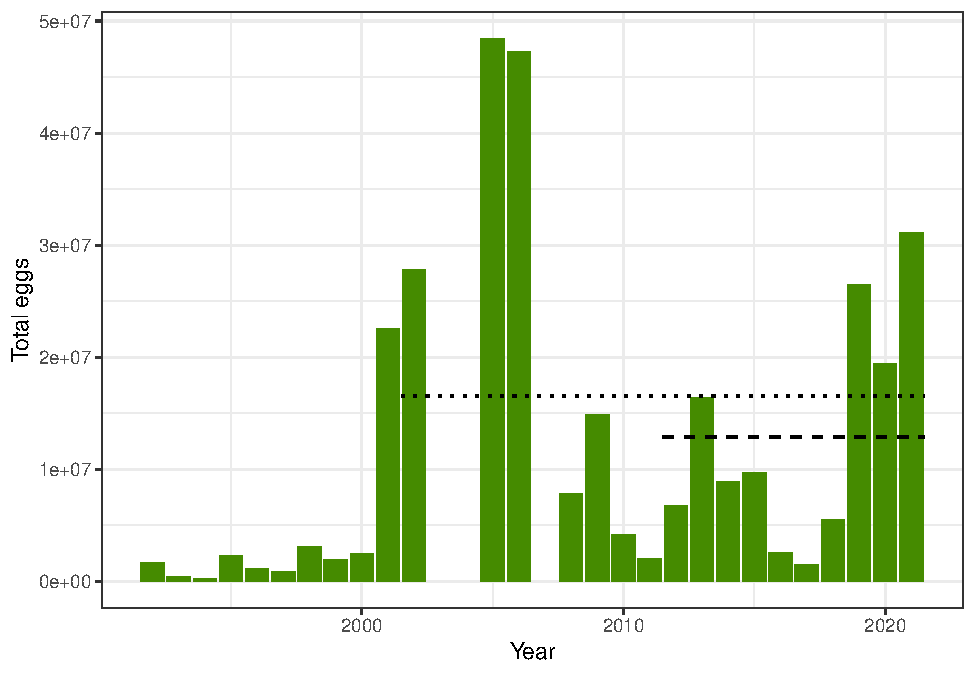
\includegraphics{_main_files/figure-latex/totaleggs-fig-1.pdf}
\caption{\label{fig:totaleggs-fig}Potential Total Eggs in the Upper Sacramento}
\end{figure}

\begin{figure}
\centering
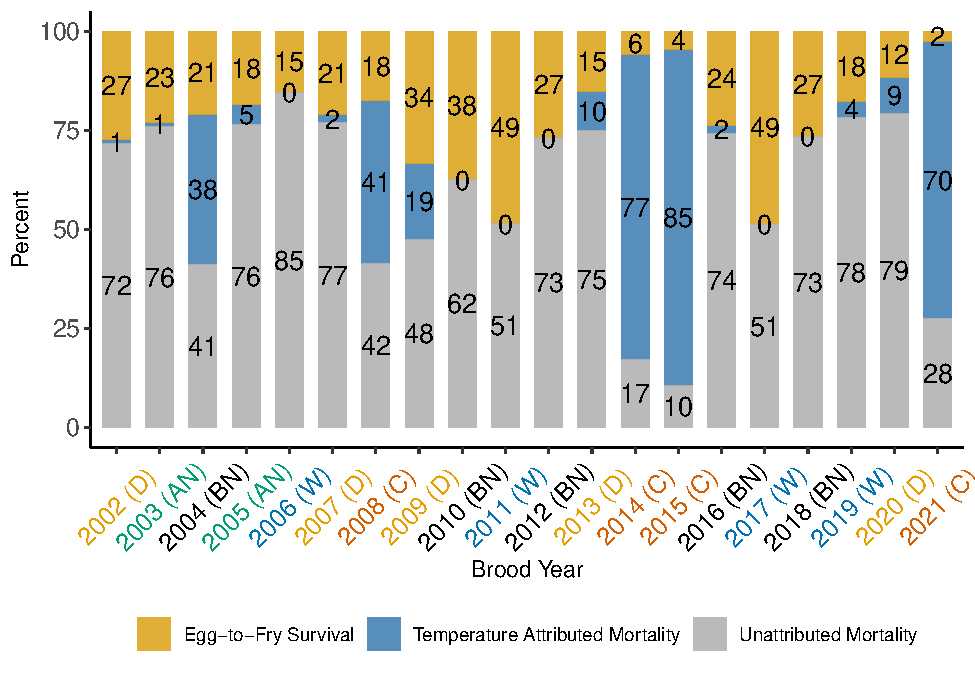
\includegraphics{_main_files/figure-latex/TDM-etf-fig-1.pdf}
\caption{\label{fig:TDM-etf-fig}Annual Percent of Egg to Fry Survival, Temperature-Dependent Mortality, and Unattributed Survival from 2002 to 2021. Labels in parentheses indicate Water Year Type.}
\end{figure}

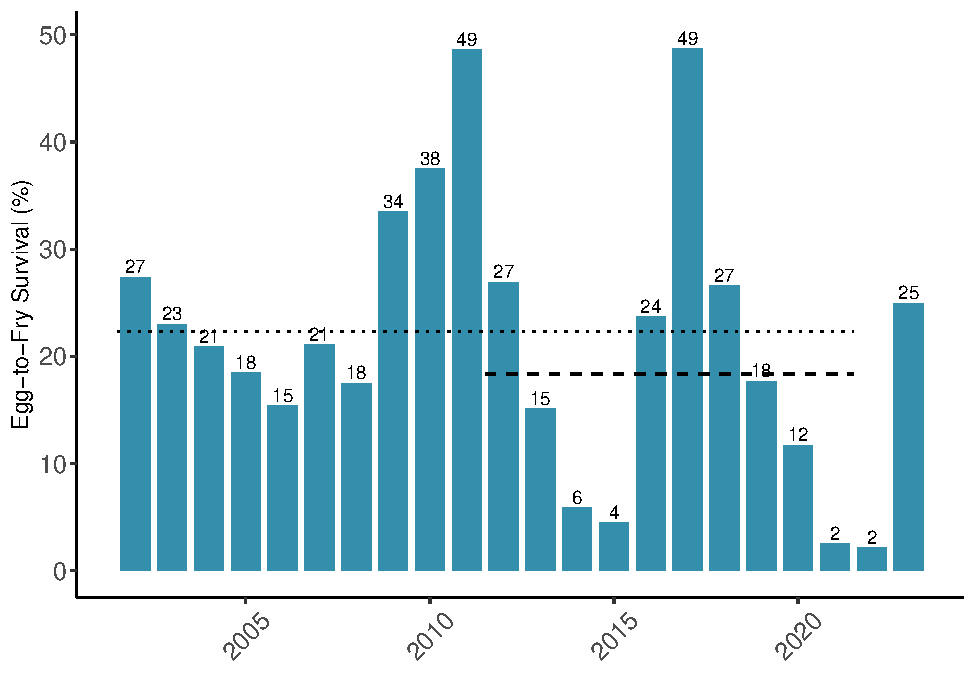
\includegraphics{_main_files/figure-latex/ETFSurv-fig-1.pdf}

SacPAS Fish Model Results for Temperature Exposure (Plot)

\hypertarget{emergence}{%
\subsection{Emergence}\label{emergence}}

\textbf{Placeholder for SacPAS fish model output for emergence timing}

SacPAS fish model estimates for emergence:

\begin{itemize}
\tightlist
\item
  \textbf{First occupancy:}
\item
  \textbf{Emergence:}
  - \textbf{First:}
  - \textbf{Mean:}
  - \textbf{Last:}
\end{itemize}

SacPAS Fish Model Results for Redd Occupation and Emergency Timing (Plot)

\hypertarget{redd-dewatering}{%
\subsection{Redd Dewatering}\label{redd-dewatering}}

I don't know if these two are the same redd (redd ID has 2 numbers switched around)
What is the unit for water depth?

\begin{itemize}
\tightlist
\item
  2 redds were dewatered in report\_year (Table \ref{tab:dewateredRedds}).
\end{itemize}

\begin{table}
\centering
\caption{Dewatered Redds in 2021}
\centering
\begin{tabular}[t]{lrlrr}
\hline
Date & River Mile & River Section & Water Depth & Flow at Keswick Dam (cfs)\\
\hline
2021-08-25 & 297.5 & Hwy 44 Brg to A.C.I.D Dam & 0 & 7290\\
\hline
2021-08-25 & 297.5 & Hwy 44 Brg to A.C.I.D Dam & 0 & 7290\\
\hline
\end{tabular}
\end{table}

\hypertarget{upper-sacramento-juveniles}{%
\chapter{Upper Sacramento Juveniles}\label{upper-sacramento-juveniles}}

This section describes environmental attributes associated with and responses during the out-migrating juvenile life stage in the Upper Sacramento River.

\hypertarget{habitat-attributes-1}{%
\section{Habitat Attributes}\label{habitat-attributes-1}}

\hypertarget{environmental-drivers-1}{%
\section{Environmental Drivers}\label{environmental-drivers-1}}

\hypertarget{flow}{%
\subsection{Flow}\label{flow}}

\label{fig:KWKBNDflowjuv-fig}Daily Flows (cfs) at Sacramento River at Keswick (KWK) and Sacramento River at Bend Bridge (BND) in July through September 2021 and over the 10-year average

\begin{table}
\centering
\caption{Mean, Maximum, Minimum Monthly Flows (cfs) at Sacramento River at Keswick (KWK) and Sacramento River at Bend Bridge (BND) in July through December 2021}
\centering
\begin{tabular}[t]{rllrrr}
\hline
Year & Month & Station & Mean & Min & Max\\
\hline
2021 & July & BND & 9642.1 & 9030 & 10600\\
\hline
2021 & August & BND & 8334.2 & 6840 & 9670\\
\hline
2021 & September & BND & 7072.0 & 6840 & 7300\\
\hline
2021 & October & BND & 13618.0 & 6220 & 36800\\
\hline
2021 & November & BND & 8279.9 & 4260 & 17700\\
\hline
2021 & December & BND & 10327.5 & 4220 & 26600\\
\hline
2021 & July & KWK & 9510.2 & 8740 & 10800\\
\hline
2021 & August & KWK & 8102.0 & 6610 & 9500\\
\hline
2021 & September & KWK & 6899.8 & 5310 & 8500\\
\hline
2021 & October & KWK & 6160.1 & 5120 & 7330\\
\hline
2021 & November & KWK & 4027.1 & 3070 & 5080\\
\hline
2021 & December & KWK & 3431.0 & 3040 & 3970\\
\hline
\end{tabular}
\end{table}

\begin{itemize}
\tightlist
\item
  \textbf{Keswick:} Peak flows were \textbf{\ensuremath{1.08\times 10^{4}}} cfs and occurred in \textbf{7}. The highest mean flows were \textbf{9510.2} cfs and occurred in \textbf{7}.
\item
  \textbf{Bend Bridge:} Peak flows were \textbf{\ensuremath{3.68\times 10^{4}}} cfs and occurred in \textbf{10}. The highest mean flows were \textbf{\ensuremath{1.3618\times 10^{4}}} cfs and occurred in \textbf{10}.
\end{itemize}

\hypertarget{water-temperature-1}{%
\subsection{Water Temperature}\label{water-temperature-1}}

\label{fig:wtempBND-fig}Daily Water Temperature (degF) at Sacramento River at Bend (BND) in 2021 and 10-year average between July and December.

\begin{table}
\centering
\caption{Mean, Maximum, Minimum Monthly Water Temperature (degF) at Sacramento River at Bend Bridge (BND) in July through December 2021}
\centering
\begin{tabular}[t]{rllrrr}
\hline
Year & Month & Station & Mean & Min & Max\\
\hline
2021 & July & BND & 59.3 & 55.9 & 62.6\\
\hline
2021 & August & BND & 59.2 & 56.0 & 62.2\\
\hline
2021 & September & BND & 60.9 & 58.7 & 63.0\\
\hline
2021 & October & BND & 59.5 & 57.1 & 61.8\\
\hline
2021 & November & BND & 54.0 & 45.2 & 60.6\\
\hline
2021 & December & BND & 50.4 & 45.6 & 55.6\\
\hline
\end{tabular}
\end{table}

\textbf{Summary}

\begin{itemize}
\tightlist
\item
  In 2021 water temperature was below average for most of the season between July and December.
\item
  \textbf{Sacramento River at Bend Bridge:} Maximum water temperature was \textbf{63} degrees F and occurred in \textbf{9}. The highest mean water temperature was \textbf{60.9} degrees F and occurred in \textbf{9}.
\end{itemize}

\hypertarget{dissolved-oxygen}{%
\subsection{Dissolved Oxygen}\label{dissolved-oxygen}}

\label{fig:doBNDjuv-fig}Daily Dissolved Oxygen (mg/L) at Sacramento River at Bend Bridge (BND) in July through December 2021 and 10-year average.

\begin{table}
\centering
\caption{Mean, Maximum, Minimum Monthly Dissolved Oxygen (mg/L) at Sacramento River at Bend Bridge (BND) in July through December 2021 . Days less than 6 mg/L indicates the number of days per month that experienced at least 1 hour where DO was less than 6 mg/L.}
\centering
\begin{tabular}[t]{rllrrrr}
\hline
Year & Month & Station & Mean & Min & Max & Days < 6mg/L\\
\hline
2021 & July & BND & 11.8 & 1.2 & 17.5 & 2\\
\hline
2021 & August & BND & 10.3 & 1.7 & 29.7 & 12\\
\hline
2021 & September & BND & 3.5 & 0.1 & 10.9 & 30\\
\hline
2021 & October & BND & 10.3 & 0.3 & 13.5 & 5\\
\hline
2021 & November & BND & 10.9 & 3.4 & 15.5 & 1\\
\hline
2021 & December & BND & 12.2 & 11.1 & 13.6 & 0\\
\hline
\end{tabular}
\end{table}

\textbf{Summary}

\begin{itemize}
\tightlist
\item
  \textbf{Sacramento River at Bend Bridge:} Minimum dissolved oxygen was \textbf{0.1} mg/L and occurred in \textbf{9}. The lowest mean dissolved oxygen was \textbf{3.5} mg/L and occurred in \textbf{9}.
\end{itemize}

\hypertarget{turbidity}{%
\subsection{Turbidity}\label{turbidity}}

\label{fig:TurbBNDRDB-fig}Daily Turbidity at Sacramento River at Bend Bridge (BND) and Red Bluff Diversion Dam (RDB) in 2021 and 10-year average between July and December. Turbidity data have not undergone QC, other than values filtered to less than 300 NTU.

\begin{table}
\centering
\caption{Mean, Maximum, Minimum Monthly Turbidity (NTU) at Sacramento River at Bend Bridge (BND) and Red Bluff Diversion Dam (RDB) in July through December 2021}
\centering
\begin{tabular}[t]{rllrrr}
\hline
Year & Month & Station & Mean & Min & Max\\
\hline
2021 & July & BND & 76.0 & 0.5 & 2565.5\\
\hline
2021 & August & BND & 30.3 & 0.1 & 1310.7\\
\hline
2021 & September & BND & 741.1 & 0.1 & 2621.3\\
\hline
2021 & October & BND & 182.8 & 1.3 & 1140.2\\
\hline
2021 & November & BND & 46.9 & 1.0 & 1138.1\\
\hline
2021 & December & BND & 73.8 & 3.6 & 990.1\\
\hline
2021 & July & RDB & 11.6 & 9.6 & 13.5\\
\hline
2021 & August & RDB & 11.1 & 9.0 & 13.2\\
\hline
2021 & September & RDB & 8.8 & 6.0 & 11.5\\
\hline
2021 & October & RDB & 9.5 & 5.2 & 13.2\\
\hline
2021 & November & RDB & 8.6 & 6.4 & 10.9\\
\hline
2021 & December & RDB & 10.2 & 5.9 & 14.4\\
\hline
\end{tabular}
\end{table}

\textbf{Summary}

\begin{itemize}
\tightlist
\item
  \textbf{Sacramento River at Bend Bridge:} Minimum turbidity was \textbf{0.1} FNU and occurred in \textbf{8} and \textbf{9}. The lowest mean turbidity was \textbf{30.3} FNU and occurred in \textbf{8}. Turbidity was below average in parts of August and September and similar at other times of the season.
\item
  \textbf{Red Bluff Diversion Dam:} Minimum turbidity was \textbf{5.2} FNU and occurred in \textbf{10}. The lowest mean turbidity was \textbf{8.6} FNU and occurred in \textbf{11}. Turbidity was below average between September and mid-December and similar at other times of the season
\end{itemize}

\hypertarget{biological-response-2}{%
\section{Biological Response}\label{biological-response-2}}

\hypertarget{fry-abundance}{%
\subsection{Fry abundance}\label{fry-abundance}}

\hypertarget{estimated-fry-passage-at-rbdd---placeholder---use-report-or-raw-data}{%
\subsubsection{Estimated Fry Passage at RBDD - Placeholder - use Report or raw data?}\label{estimated-fry-passage-at-rbdd---placeholder---use-report-or-raw-data}}

\begin{itemize}
\tightlist
\item
  Percent Fry Passage at RBDD (fry/fry+smolts)
\end{itemize}

\hypertarget{fry-equivalent-jpi}{%
\subsubsection{Fry-equivalent JPI}\label{fry-equivalent-jpi}}

\begin{figure}
\centering
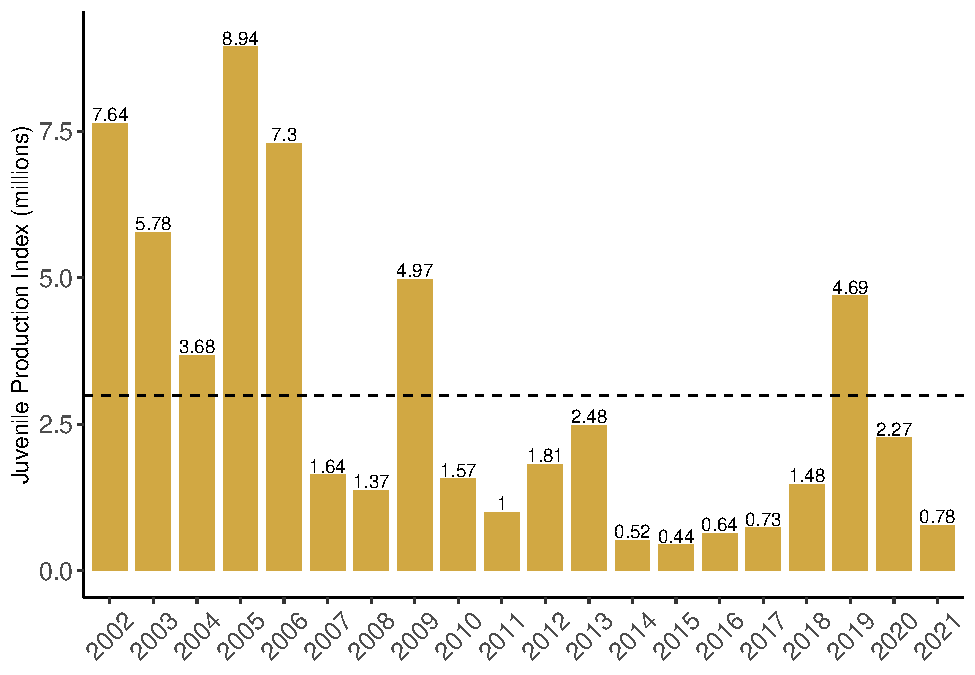
\includegraphics{_main_files/figure-latex/JPI-fig-1.pdf}
\caption{\label{fig:JPI-fig}Annual JPI from 2002 to 2021}
\end{figure}

\begin{itemize}
\item
  By year
\item
  RBDD RST Data
\item
  \textbf{Juvenile Production Index} JPI in 2021 was below the average JPI between 2002 and 2021 at 0.779427.
\end{itemize}

\begin{enumerate}
\def\labelenumi{\arabic{enumi}.}
\setcounter{enumi}{1}
\tightlist
\item
  Condition/ Growth
\end{enumerate}

\begin{itemize}
\tightlist
\item
  Fork length by year
\end{itemize}

\begin{enumerate}
\def\labelenumi{\arabic{enumi}.}
\setcounter{enumi}{2}
\tightlist
\item
  Migration Timing
\end{enumerate}

\begin{itemize}
\tightlist
\item
  RBDD RST Data
\end{itemize}

\begin{enumerate}
\def\labelenumi{\arabic{enumi}.}
\setcounter{enumi}{3}
\tightlist
\item
  Fry-to-Smolt Survival
\end{enumerate}

\begin{itemize}
\tightlist
\item
  Model?
\end{itemize}

\hypertarget{stranding}{%
\subsection{Stranding}\label{stranding}}

A total of 383 juveniles were stranded.

\begin{table}
\centering
\caption{Juvenile Stranding in 2021}
\centering
\begin{tabular}[t]{lrllrrl}
\hline
Date & Section Number & Section Name & River Miles & Count & Flow (cfs) & Flow Gage\\
\hline
2021-08-26 & 2 & Hwy 44 Brg to A.C.I.D Dam & 298-296 & 4 & 6699 & KWK\\
\hline
2021-11-08 & 2 & Hwy 44 Brg to A.C.I.D Dam & 298-296 & 34 & 3751 & KWK\\
\hline
2021-11-09 & 2 & Hwy 44 Brg to A.C.I.D Dam & 298-296 & 65 & 3747 & KWK\\
\hline
2021-11-01 & 3 & Clear Crk. Powerlines to Hwy 44 Brg & 296-288 & 12 & 4982 & KWK\\
\hline
2021-10-28 & 4 & Balls Ferry Brg to Clear Crk Powerlines & 288-276 & 9 & 5761 & KWK\\
\hline
2021-11-03 & 4 & Balls Ferry Brg to Clear Crk Powerlines & 288-276 & 75 & 4458 & KWK\\
\hline
2021-11-10 & 4 & Balls Ferry Brg to Clear Crk Powerlines & 288-276 & 27 & 3582 & KWK\\
\hline
2021-11-18 & 4 & Balls Ferry Brg to Clear Crk Powerlines & 288-276 & 11 & 3268 & KWK\\
\hline
2021-10-27 & 8 & RBDD to Bend Brg & 257-242 & 71 & 8500 & BND\\
\hline
2021-11-01 & 8 & RBDD to Bend Brg & 257-242 & 20 & 6268 & BND\\
\hline
2021-11-02 & 8 & RBDD to Bend Brg & 257-242 & 46 & 6824 & BND\\
\hline
2021-11-04 & 8 & RBDD to Bend Brg & 257-242 & 1 & 5814 & BND\\
\hline
2021-11-16 & 8 & RBDD to Bend Brg & 257-242 & 4 & 4723 & BND\\
\hline
2021-12-18 & 8 & RBDD to Bend Brg & 257-242 & 2 & 6198 & BND\\
\hline
2021-12-27 & 8 & RBDD to Bend Brg & 257-242 & 2 & 8980 & BND\\
\hline
\end{tabular}
\end{table}

\hypertarget{condition}{%
\subsection{Condition}\label{condition}}

\hypertarget{rbdd-size}{%
\subsubsection{RBDD Size}\label{rbdd-size}}

\begin{figure}
\centering
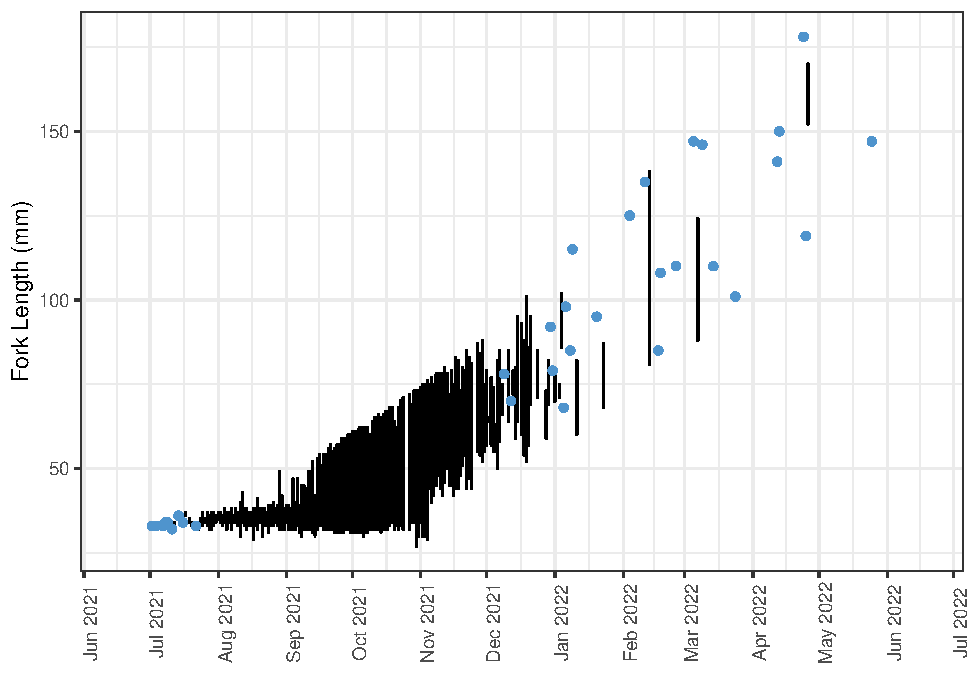
\includegraphics{_main_files/figure-latex/rbdd-fl-fig-1.pdf}
\caption{\label{fig:rbdd-fl-fig}Fork Length Distribution over Time, RBDD RST}
\end{figure}

\begin{figure}
\centering
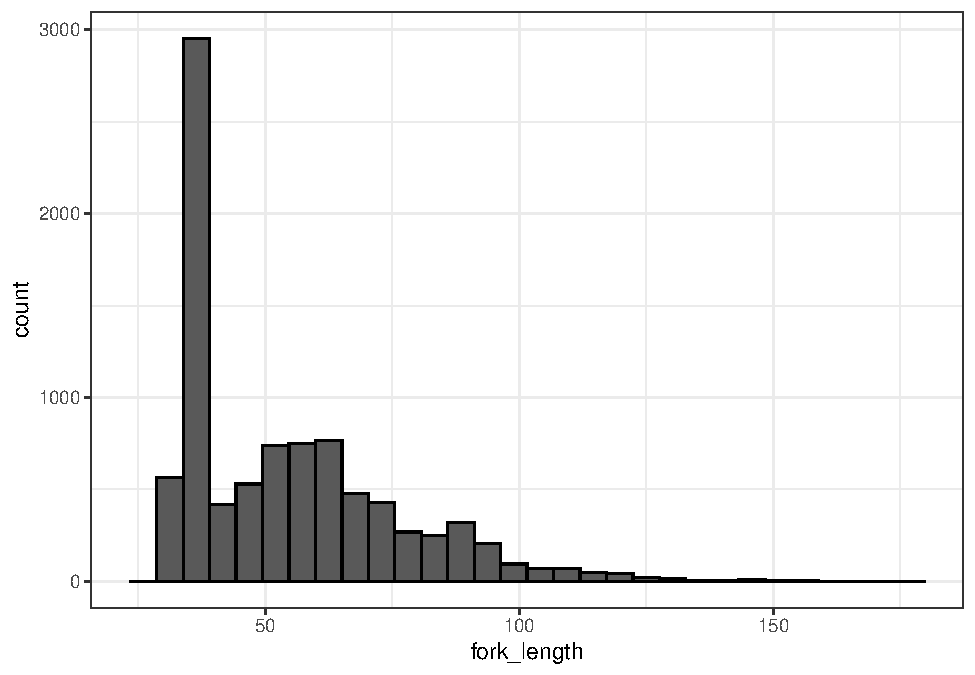
\includegraphics{_main_files/figure-latex/rbdd-flhist-fig-1.pdf}
\caption{\label{fig:rbdd-flhist-fig}Fork Length Distribution over Time, RBDD RST}
\end{figure}

\hypertarget{middle-and-lower-sacramento-juveniles}{%
\chapter{Middle and Lower Sacramento Juveniles}\label{middle-and-lower-sacramento-juveniles}}

This section describes environmental attributes associated with and responses during the out-migrating juvenile life stage in the Lower and Middle Sacramento River.

\hypertarget{habitat-attributes-2}{%
\section{Habitat Attributes}\label{habitat-attributes-2}}

\begin{enumerate}
\def\labelenumi{\arabic{enumi}.}
\item
  Habitat Capacity (Floodplain Connectivity)
\item
  Habitat Capacity: Depth/Shallow Water
\item
  In-Stream Habitat Capacity
\end{enumerate}

\hypertarget{storage-and-flows}{%
\subsection{Storage and Flows}\label{storage-and-flows}}

\begin{enumerate}
\def\labelenumi{\arabic{enumi}.}
\item
  Shasta Storage/Hydrology
\item
  Flows: Migration Cues
\end{enumerate}

\hypertarget{flow-conditions-on-the-middle-and-lower-sacramento-river}{%
\subsubsection{Flow Conditions on the Middle and Lower Sacramento River}\label{flow-conditions-on-the-middle-and-lower-sacramento-river}}

\label{fig:HMCWLKVONflow-fig}Daily Flows (cfs) at Sacramento River at Hamilton City (HMC), Sacramento River at Wilkins Slough (WLK) and Sacramento River at Verona (VON) from September 2021 through March 2022 and over the 10-year average

\begin{table}
\centering
\caption{Mean, Maximum and Minimum Monthly Flows (cfs) at Sacramento River at Hamilton City (HMC), Sacramento River at Wilkins Slough (WLK) and Sacramento River at Verona (VON) from September 2021  through March 2022}
\centering
\begin{tabular}[t]{rllrrr}
\hline
Year & Month & Station & Mean & Min & Max\\
\hline
2021 & September & HMC & 5885.7 & 5590 & 6182\\
\hline
2021 & October & HMC & 13842.8 & 5945 & 47509\\
\hline
2021 & November & HMC & 7181.8 & 3983 & 17544\\
\hline
2021 & December & HMC & 11421.0 & 3400 & 29442\\
\hline
2022 & January & HMC & 7669.2 & 4678 & 12005\\
\hline
2022 & February & HMC & 4326.8 & 3744 & 4934\\
\hline
2022 & March & HMC & 3983.1 & 3615 & 4333\\
\hline
2021 & September & WLK & 5605.0 & 5290 & 5920\\
\hline
2021 & October & WLK & 11000.4 & 5650 & 25100\\
\hline
2021 & November & WLK & 7160.0 & 4370 & 12700\\
\hline
2021 & December & WLK & 9375.3 & 3990 & 20600\\
\hline
2022 & January & WLK & 7715.4 & 5190 & 12000\\
\hline
2022 & February & WLK & 4732.0 & 4060 & 5400\\
\hline
2022 & March & WLK & 4200.0 & 3930 & 4470\\
\hline
2021 & September & VON & 7827.2 & 7160 & 8420\\
\hline
2021 & October & VON & 18089.0 & 7110 & 35500\\
\hline
2021 & November & VON & 8051.0 & 5480 & 12900\\
\hline
2021 & December & VON & 15431.8 & 5500 & 31900\\
\hline
2022 & January & VON & 14467.4 & 9010 & 23200\\
\hline
2022 & February & VON & 10197.1 & 9610 & 11500\\
\hline
2022 & March & VON & 8856.6 & 7490 & 11200\\
\hline
\end{tabular}
\end{table}

\hypertarget{juvenile-wrcs-rescued-during-stranding-surveys}{%
\subsubsection{Juvenile WRCS Rescued During Stranding Surveys}\label{juvenile-wrcs-rescued-during-stranding-surveys}}

Fish were not stranded in the Middle to Lower Sacramento River for Brood Year 2021.

\textbf{Summary}

\begin{itemize}
\item
  \textbf{Hamilton City:} Peak flows were \textbf{\ensuremath{4.7509\times 10^{4}}} cfs and occurred in \textbf{10}. The highest mean flows were \textbf{\ensuremath{1.38428\times 10^{4}}} cfs and occurred in \textbf{10}.
\item
  \textbf{Wilkins Slough:} Peak flows were \textbf{\ensuremath{2.51\times 10^{4}}} cfs and occurred in \textbf{10}. The highest mean flows were \textbf{\ensuremath{1.10004\times 10^{4}}} cfs and occurred in \textbf{10}.
\item
  \textbf{Verona:} Peak flows were \textbf{\ensuremath{3.55\times 10^{4}}} cfs and occurred in \textbf{10}. The highest mean flows were \textbf{\ensuremath{1.8089\times 10^{4}}} cfs and occurred in \textbf{10}.
\end{itemize}

\hypertarget{environmental-drivers-2}{%
\subsection{Environmental Drivers}\label{environmental-drivers-2}}

\hypertarget{turbidity-1}{%
\subsubsection{Turbidity}\label{turbidity-1}}

\label{fig:RDBFPTDO-fig}Daily Turbidity at Red Bluff Diversion Dam (RDB) and Sacramento River at Freeport (FPT) from September 2021 through March 2022

\begin{table}
\centering
\caption{Mean, Maximum, Minimum Monthly Flows (cfs) at Red Bluff Diversion Dam (RDB) and Sacramento River at Freeport (FPT) from September 2021 through March 2022}
\centering
\begin{tabular}[t]{rllrrr}
\hline
Year & Month & Station & Mean & Min & Max\\
\hline
2021 & September & RDB & 8.8 & 6.0 & 11.5\\
\hline
2021 & October & RDB & 9.5 & 5.2 & 13.2\\
\hline
2021 & November & RDB & 8.6 & 6.4 & 10.9\\
\hline
2021 & December & RDB & 10.3 & 5.9 & 14.5\\
\hline
2022 & January & RDB & 14.0 & 11.1 & 16.9\\
\hline
2022 & February & RDB & 14.4 & 11.4 & 17.3\\
\hline
2022 & March & RDB & 9.7 & 4.3 & 15.3\\
\hline
2021 & September & FPT & 2.6 & 0.8 & 5.2\\
\hline
2021 & October & FPT & 47.7 & 1.0 & 123.0\\
\hline
2021 & November & FPT & 10.1 & 3.4 & 24.0\\
\hline
2021 & December & FPT & 44.2 & 2.3 & 107.0\\
\hline
2022 & January & FPT & 14.5 & 1.6 & 30.3\\
\hline
2022 & February & FPT & 7.3 & 3.0 & 11.8\\
\hline
2022 & March & FPT & 5.1 & 1.8 & 10.1\\
\hline
\end{tabular}
\end{table}

\textbf{Summary}

\begin{itemize}
\tightlist
\item
  \textbf{Red Bluff Diversion Dam:} Minimum turbidity was \textbf{4.3} FNU and occurred in \textbf{3}. The lowest mean turbidity was \textbf{8.6} FNU and occurred in \textbf{11}.
\item
  \textbf{Sacramento River at Freeport:} Minimum turbidity was \textbf{0.8} FNU and occurred in \textbf{9}. The lowest mean turbidity was \textbf{2.6} FNU and occurred in \textbf{9}.
\end{itemize}

\hypertarget{water-temperature-2}{%
\subsubsection{Water Temperature}\label{water-temperature-2}}

\begin{table}
\centering
\caption{Mean, Maximum, Minimum Monthly Water Temperature (°F) at Sacramento River Below Wilkins Slough (WLK) in September 2021 through March 2022 . Days > 63°F indicates the number of days per month that experienced at least 1 hour where Water Temperature was greater than 63°F.}
\centering
\begin{tabular}[t]{rllrrrr}
\hline
Year & Month & Station & Mean & Min & Max & Water Temp < 63 Degf\\
\hline
2021 & September & WLK & 69.5 & 63.8 & 90.7 & 30\\
\hline
2021 & October & WLK & 61.2 & 57.3 & 71.7 & 8\\
\hline
2021 & November & WLK & 56.8 & 52.4 & 62.0 & 0\\
\hline
2021 & December & WLK & 49.7 & 45.1 & 54.9 & 0\\
\hline
2022 & January & WLK & 48.7 & 44.8 & 51.0 & 0\\
\hline
2022 & February & WLK & 51.9 & 47.0 & 56.7 & 0\\
\hline
2022 & March & WLK & 58.8 & 53.0 & 66.7 & 8\\
\hline
\end{tabular}
\end{table}

\textbf{Summary}

\begin{itemize}
\tightlist
\item
  Maximum water temperature was \textbf{90.7} degrees F and occurred in \textbf{9}. The highest mean water temperature was \textbf{69.5} degrees F and occurred in \textbf{9}.
\item
  The month with greatest days exceeding 63 degrees F (\textbf{30} days) was \textbf{9}.
\end{itemize}

\hypertarget{dissolved-oxygen-1}{%
\subsubsection{Dissolved Oxygen}\label{dissolved-oxygen-1}}

\begin{table}
\centering
\caption{Mean, Maximum, Minimum Monthly Flows (cfs) at Red Bluff Diversion Dam (RDB) and Sacramento River at Hood (SRH) in 2021 - 2022 . Days less than 6 mg/L indicates the number of days per month that experienced at least 1 hour where DO was less than 6 mg/L.}
\centering
\begin{tabular}[t]{rllrrrr}
\hline
Year & Month & Station & Mean & Min & Max & Do < 6mg/L\\
\hline
2021 & September & RDB & 8.4 & 6.0 & 11.5 & 0\\
\hline
2021 & October & RDB & 9.9 & 5.2 & 13.2 & 5\\
\hline
2021 & November & RDB & 8.5 & 6.4 & 10.9 & 0\\
\hline
2021 & December & RDB & 10.2 & 5.9 & 14.5 & 1\\
\hline
2022 & January & RDB & 14.2 & 11.1 & 16.9 & 0\\
\hline
2022 & February & RDB & 14.5 & 11.4 & 17.3 & 0\\
\hline
2022 & March & RDB & 8.3 & 4.3 & 15.3 & 17\\
\hline
2021 & September & SRH & 8.2 & 7.6 & 9.2 & 0\\
\hline
2021 & October & SRH & 8.8 & 6.4 & 10.0 & 0\\
\hline
2021 & November & SRH & 8.9 & 7.1 & 10.1 & 0\\
\hline
2021 & December & SRH & 10.1 & 9.5 & 10.7 & 0\\
\hline
2022 & January & SRH & 11.0 & 10.6 & 11.4 & 0\\
\hline
2022 & February & SRH & 10.9 & 10.2 & 11.7 & 0\\
\hline
2022 & March & SRH & 9.9 & 8.5 & 11.1 & 0\\
\hline
\end{tabular}
\end{table}

\textbf{Summary}

\begin{itemize}
\tightlist
\item
  \textbf{Sacramento River at Bend Bridge:} Minimum dissolved oxygen was \textbf{4.3} mg/L and occurred in \textbf{3}. The lowest mean dissolved oxygen was \textbf{8.3} mg/L and occurred in \textbf{3}.
\item
  \textbf{Sacramento River at Hood:} Minimum dissolved oxygen was \textbf{6.4} mg/L and occurred in \textbf{10}. The lowest mean dissolved oxygen was \textbf{8.2} mg/L and occurred in \textbf{9}.
\end{itemize}

\hypertarget{rearing-habitat-capacity}{%
\section{Rearing Habitat Capacity}\label{rearing-habitat-capacity}}

\hypertarget{biological-response-3}{%
\section{Biological Response}\label{biological-response-3}}

Monitoring Sources for abundance, growth/size, migration timing/duration

\begin{itemize}
\tightlist
\item
  Sac Trawl
\item
  Tisdale Weir
\item
  Knights Landing
\item
  GCID
\item
  DJFMP
\item
  Yolo Bypass
\item
  Chipps Island Trawl (Exit)
\item
  Genetic (Chipps, SWP/CVP, Knights Landing, Yolo Bypass)
\end{itemize}

\textbf{Data Sources}

\begin{itemize}
\tightlist
\item
  JPE, Smolt survival from JPE Letters (link)
\item
\end{itemize}

\hypertarget{juvenile-production-estimate-abundance}{%
\subsection{Juvenile Production Estimate (Abundance)}\label{juvenile-production-estimate-abundance}}

\begin{figure}
\centering
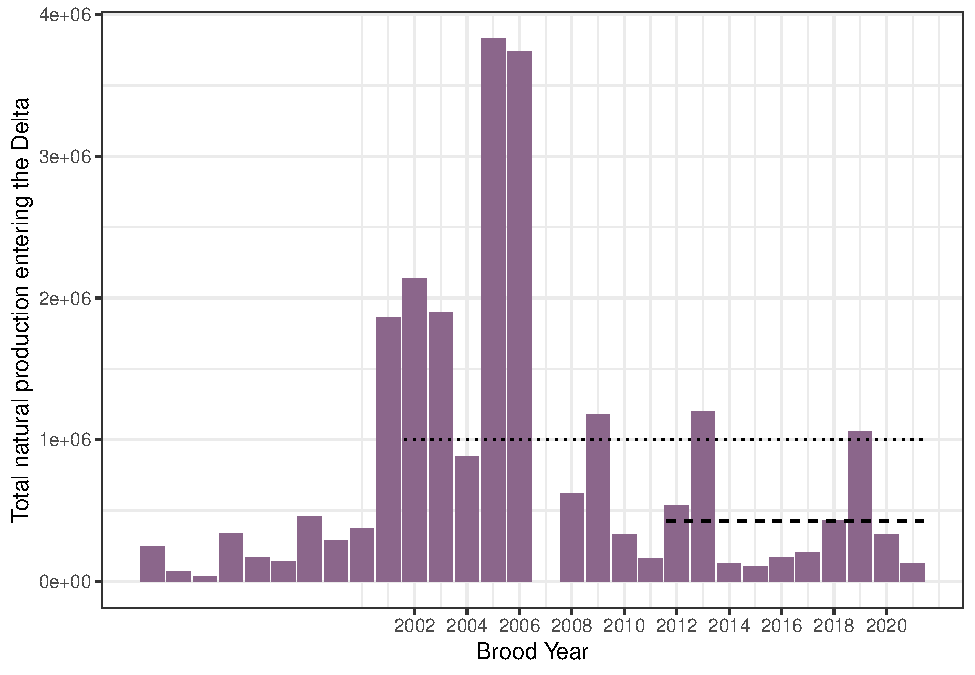
\includegraphics{_main_files/figure-latex/jpe-fig-1.pdf}
\caption{\label{fig:jpe-fig}Total Natural production entering the Delta (JPE)}
\end{figure}

\begin{figure}
\centering
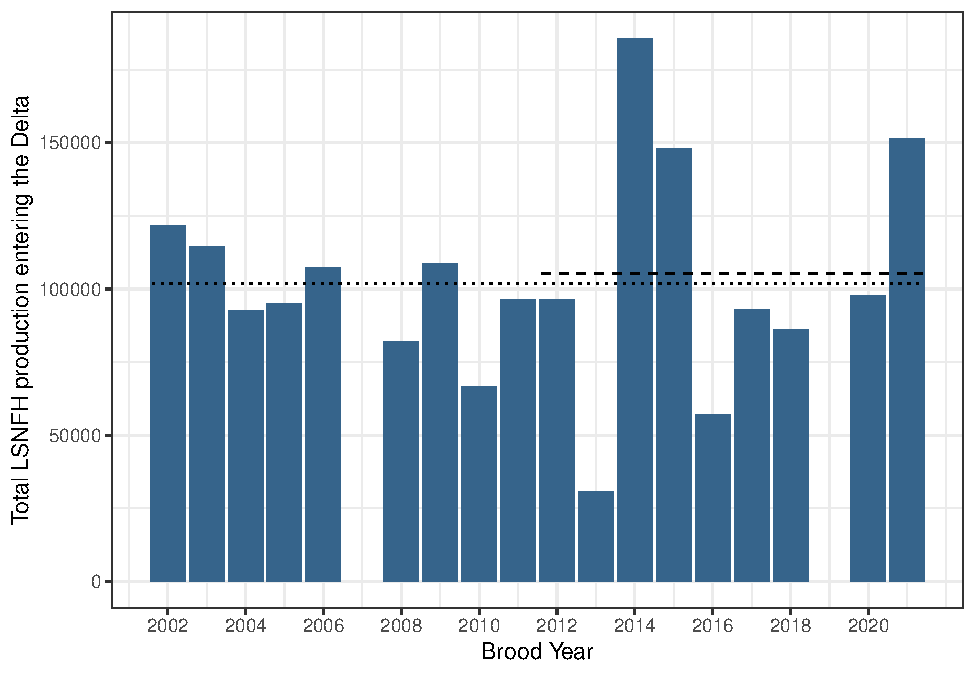
\includegraphics{_main_files/figure-latex/jpeH-fig-1.pdf}
\caption{\label{fig:jpeH-fig}Total Hatchery Production entering the Delta (Hatchery JPE)}
\end{figure}

\hypertarget{smolt-survival}{%
\subsection{Smolt Survival}\label{smolt-survival}}

\hypertarget{jpe-letter}{%
\subsubsection{JPE Letter}\label{jpe-letter}}

Natural-origin smolt survival is calculated at the Tower Bridge from acoustically tagged hatchery fish that are released at RBDD.

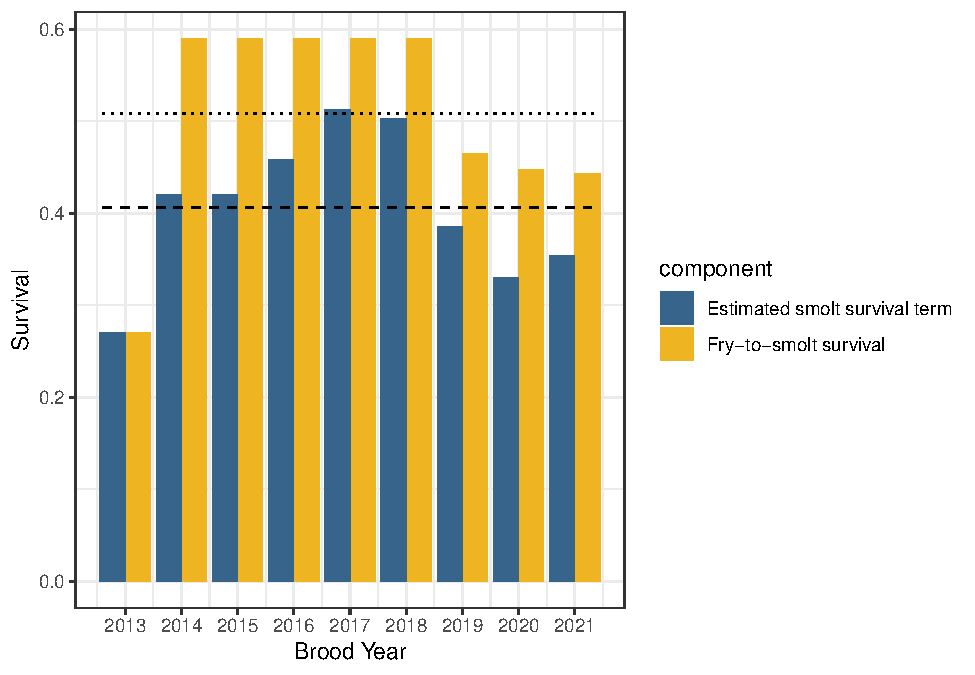
\includegraphics{_main_files/figure-latex/smoltsurvival-fig-1.pdf}
\#\#\#\# Acoustic Tagging

Reach-specific survival

\begin{table}
\centering
\caption{Table of Hatchery WR Juvenile Survival}
\centering
\begin{tabular}[t]{lllrllr}
\hline
rel\_date & reach\_start & reach\_end & rkm\_start & ReachSurvival & CumulativeSurvival & count\\
\hline
2022-02-10 & Caldwell\_Park\_Rel & Blw\_Cypress & 551 & 0.995 (0.988, 0.998) & 1 (0, 0) & 139\\
\hline
2022-02-10 & Blw\_Cypress & Blw\_ClearCr & 544 & 0.999 (0.994, 1) & 0.964 (0.92, 0.98) & 134\\
\hline
2022-02-10 & Blw\_ClearCr & BlwCowCr & 536 & 0.999 (0.996, 1) & 0.957 (0.91, 0.98) & 133\\
\hline
2022-02-10 & BlwCowCr & Battle\_Conf & 521 & 0.999 (0.995, 1) & 0.95 (0.9, 0.98) & 132\\
\hline
2022-02-10 & Battle\_Conf & Blw\_Paynes\_Ck & 507 & 0.997 (0.995, 0.999) & 0.935 (0.88, 0.97) & 130\\
\hline
2022-02-10 & Blw\_Paynes\_Ck & Blw\_Salt & 476 & 0.996 (0.992, 0.998) & 0.863 (0.8, 0.91) & 120\\
\hline
2022-02-10 & Blw\_Salt & Mill\_Ck\_Conf & 457 & 0.999 (0.99, 1) & 0.799 (0.72, 0.86) & 111\\
\hline
2022-02-10 & Mill\_Ck\_Conf & Ord & 441 & 0.992 (0.989, 0.994) & 0.782 (0.7, 0.85) & 106\\
\hline
2022-02-10 & Ord & Colusa AC2 & 372 & 0.989 (0.984, 0.993) & 0.449 (0.36, 0.54) & 57\\
\hline
2022-02-10 & Colusa AC2 & AbvColusaBr & 319 & 0.998 (0.978, 1) & 0.252 (0.19, 0.33) & 35\\
\hline
2022-02-10 & AbvColusaBr & Colusa BC2 & 308 & 0.998 (0.947, 1) & 0.245 (0.18, 0.32) & 31\\
\hline
2022-02-10 & Colusa BC2 & AbvTisdale & 296 & 0.997 (0.988, 0.999) & 0.241 (0.18, 0.32) & 26\\
\hline
2022-02-10 & AbvTisdale & Knights\_RST & 269 & 0.995 (0.99, 0.998) & 0.224 (0.16, 0.3) & 30\\
\hline
2022-02-10 & Knights\_RST & Abv\_FremontWeir & 222 & 0.995 (0.952, 0.999) & 0.18 (0.12, 0.25) & 25\\
\hline
2022-02-10 & Abv\_FremontWeir & SacFeather & 215 & 0.995 (0.965, 0.999) & 0.174 (0.12, 0.25) & 21\\
\hline
2022-02-10 & SacFeather & Blw\_Elkhorn\_GS1 & 206 & 1 (1, 1) & 0.165 (0.11, 0.24) & 22\\
\hline
2022-02-10 & Blw\_Elkhorn\_GS1 & TowerBridge & 192 & 0.998 (0.984, 1) & 0.165 (0.11, 0.24) & 23\\
\hline
2022-02-10 & TowerBridge & SacTrawl & 172 & 1 (1, 1) & 0.158 (0.11, 0.23) & 22\\
\hline
2022-02-10 & NA & NA & 167 & NA (NA, NA) & 0.158 (0.11, 0.23) & 22\\
\hline
2022-02-10 & Freeport & Abv\_Clarksburg & 152 & 1 (1, 1) & 0.137 (0.09, 0.2) & 19\\
\hline
2022-02-10 & Abv\_Clarksburg & Hood & 148 & 1 (1, 1) & 0.137 (0.09, 0.2) & 19\\
\hline
2022-02-10 & Hood & Chipps & 138 & 0.992 (0.984, 0.996) & 0.137 (0.09, 0.2) & 19\\
\hline
2022-02-10 & Chipps & Benicia & 71 & 0.989 (0.959, 0.997) & 0.08 (0.04, 0.14) & 11\\
\hline
2022-02-10 & Benicia & GoldenGateE & 52 & 1 (1, 1) & 0.065 (0.03, 0.12) & 9\\
\hline
2022-02-10 & NA & NA & 2 & NA (NA, NA) & 0.065 (0.03, 0.12) & 2\\
\hline
2022-03-02 & Caldwell\_Park\_Rel & Blw\_Cypress & 551 & 0.996 (0.993, 0.998) & 1 (0, 0) & 430\\
\hline
2022-03-02 & Blw\_Cypress & Blw\_ClearCr & 544 & 0.999 (0.997, 1) & 0.972 (0.95, 0.98) & 418\\
\hline
2022-03-02 & Blw\_ClearCr & BlwCowCr & 536 & 1 (0.999, 1) & 0.963 (0.94, 0.98) & 414\\
\hline
2022-03-02 & BlwCowCr & Battle\_Conf & 521 & 0.998 (0.997, 0.999) & 0.958 (0.94, 0.97) & 412\\
\hline
2022-03-02 & Battle\_Conf & Blw\_Paynes\_Ck & 507 & 0.997 (0.996, 0.998) & 0.935 (0.91, 0.96) & 402\\
\hline
2022-03-02 & Blw\_Paynes\_Ck & Blw\_Salt & 476 & 0.997 (0.995, 0.998) & 0.856 (0.82, 0.89) & 368\\
\hline
2022-03-02 & Blw\_Salt & Mill\_Ck\_Conf & 457 & 0.993 (0.99, 0.996) & 0.8 (0.76, 0.84) & 344\\
\hline
2022-03-02 & Mill\_Ck\_Conf & Ord & 441 & 0.988 (0.986, 0.99) & 0.722 (0.67, 0.77) & 291\\
\hline
2022-03-02 & Ord & Colusa AC2 & 372 & 0.991 (0.988, 0.994) & 0.315 (0.27, 0.36) & 116\\
\hline
2022-03-02 & Colusa AC2 & AbvColusaBr & 319 & 0.99 (0.981, 0.995) & 0.198 (0.16, 0.24) & 85\\
\hline
2022-03-02 & AbvColusaBr & Colusa BC2 & 308 & 0.997 (0.987, 0.999) & 0.178 (0.14, 0.22) & 68\\
\hline
2022-03-02 & Colusa BC2 & AbvTisdale & 296 & 0.999 (0.995, 1) & 0.171 (0.14, 0.21) & 61\\
\hline
2022-03-02 & AbvTisdale & Knights\_RST & 269 & 0.998 (0.996, 0.999) & 0.166 (0.13, 0.2) & 69\\
\hline
2022-03-02 & Knights\_RST & Abv\_FremontWeir & 222 & 0.998 (0.981, 1) & 0.153 (0.12, 0.19) & 66\\
\hline
2022-03-02 & Abv\_FremontWeir & SacFeather & 215 & 0.998 (0.985, 1) & 0.151 (0.12, 0.19) & 58\\
\hline
2022-03-02 & SacFeather & Blw\_Elkhorn\_GS1 & 206 & 0.996 (0.989, 0.999) & 0.149 (0.12, 0.19) & 61\\
\hline
2022-03-02 & Blw\_Elkhorn\_GS1 & TowerBridge & 192 & 0.994 (0.987, 0.997) & 0.142 (0.11, 0.18) & 61\\
\hline
2022-03-02 & TowerBridge & SacTrawl & 172 & 0.985 (0.961, 0.994) & 0.126 (0.1, 0.16) & 54\\
\hline
2022-03-02 & NA & NA & 167 & NA (NA, NA) & 0.116 (0.09, 0.15) & 50\\
\hline
2022-03-02 & Freeport & Abv\_Clarksburg & 152 & 0.991 (0.964, 0.998) & 0.107 (0.08, 0.14) & 46\\
\hline
2022-03-02 & Abv\_Clarksburg & Hood & 148 & 0.995 (0.981, 0.999) & 0.102 (0.08, 0.14) & 44\\
\hline
2022-03-02 & Hood & Chipps & 138 & 0.993 (0.989, 0.996) & 0.098 (0.07, 0.13) & 42\\
\hline
2022-03-02 & Chipps & Benicia & 71 & 0.994 (0.981, 0.998) & 0.063 (0.04, 0.09) & 26\\
\hline
2022-03-02 & Benicia & GoldenGateE & 52 & 1 (1, 1) & 0.056 (0.04, 0.08) & 24\\
\hline
2022-03-02 & NA & NA & 2 & NA (NA, NA) & 0.056 (0.04, 0.08) & 11\\
\hline
\end{tabular}
\end{table}

\hypertarget{migration-timing}{%
\subsection{Migration Timing}\label{migration-timing}}

Cumulative Raw Catch: RBDD, Chipps, Tisdale, Knights, Sac Beach Seines, Sac Trawls
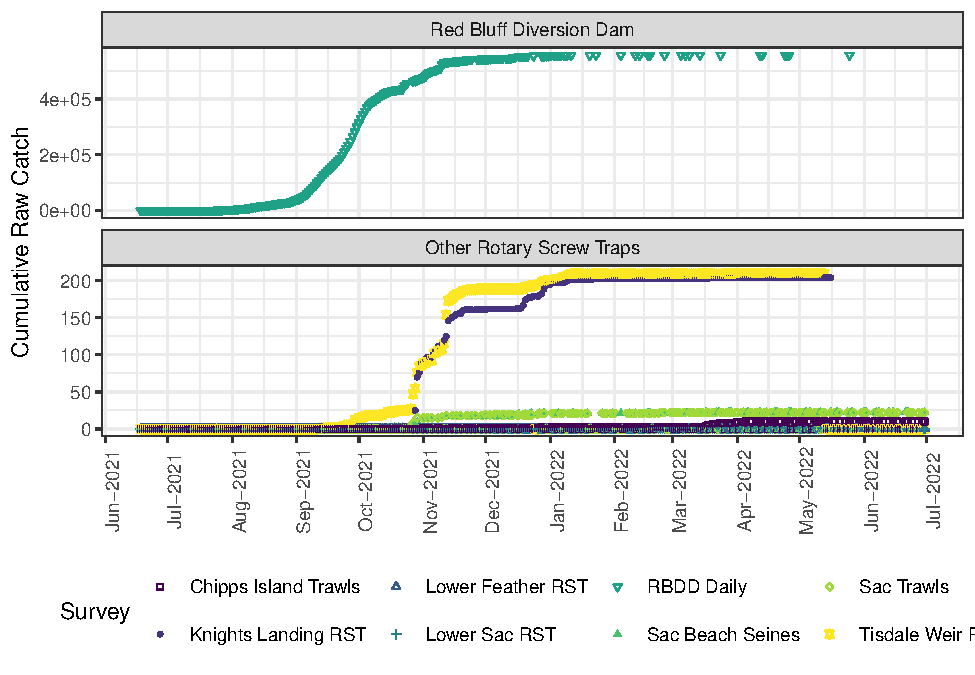
\includegraphics{_main_files/figure-latex/juvtiming-fig-1.pdf}

Median Passage Dates

Migration Timing

\hypertarget{condition-1}{%
\subsection{Condition}\label{condition-1}}

Do we want FL on any surveys?

\hypertarget{sacramento-san-joaquin-delta-juveniles}{%
\chapter{Sacramento-San Joaquin Delta Juveniles}\label{sacramento-san-joaquin-delta-juveniles}}

This section describes environmental attributes associated with and responses during the out-migrating juvenile life stage in the Sacramento-San Joaquin Delta.

\hypertarget{habitat-attributes-3}{%
\section{Habitat Attributes}\label{habitat-attributes-3}}

\begin{enumerate}
\def\labelenumi{\arabic{enumi}.}
\tightlist
\item
  Rearing Habitat Capacity (Floodplain Connectivity)
\end{enumerate}

\begin{itemize}
\tightlist
\item
  Weir overtopping
\end{itemize}

\hypertarget{food-availability}{%
\subsection{Food Availability}\label{food-availability}}

\begin{figure}
\centering
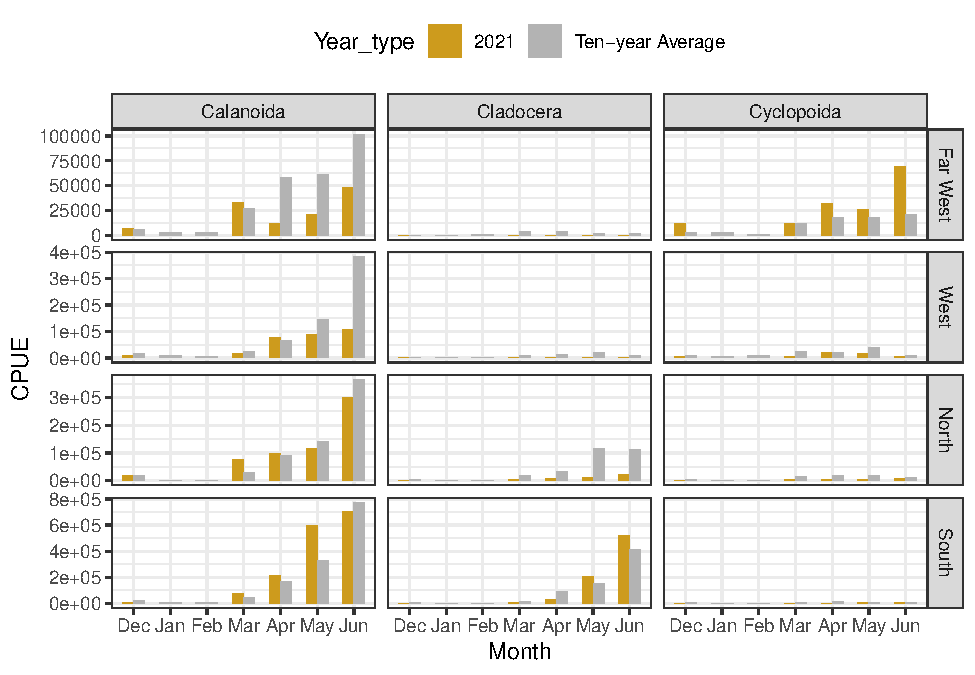
\includegraphics{_main_files/figure-latex/meso-fig-1.pdf}
\caption{\label{fig:meso-fig}Zooplankton Abundance in the Delta, December 2021 - June 2022 and 10-year average CPUE}
\end{figure}

Macrozooplankton currently lacking 2022 data

\begin{figure}
\centering
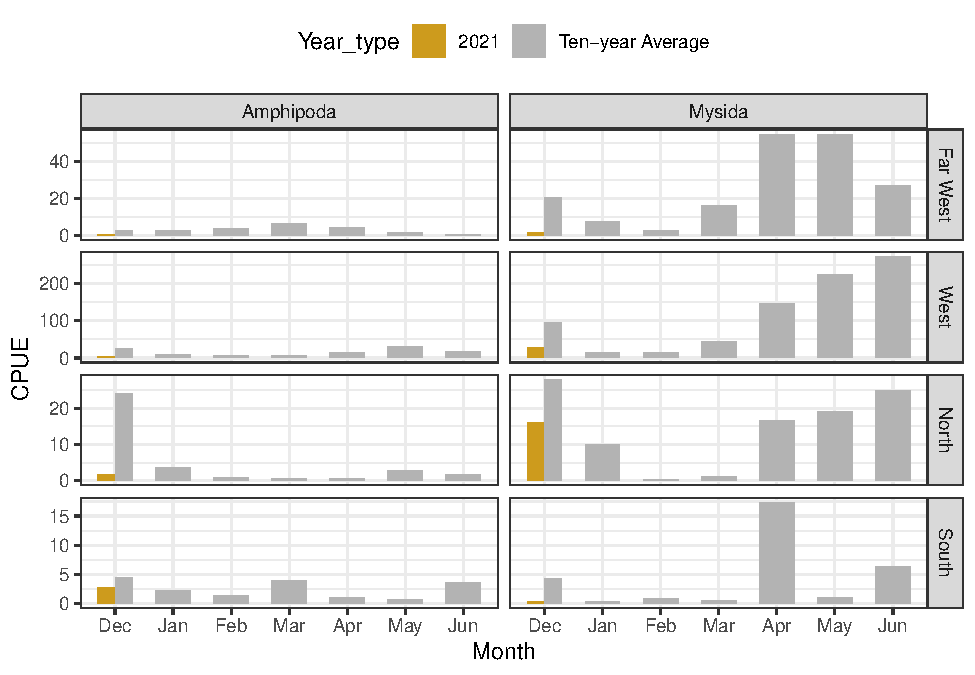
\includegraphics{_main_files/figure-latex/macro-fig-1.pdf}
\caption{\label{fig:macro-fig}Amphipod and Mysid Abundance in the Delta, December 2021 - June 2022 and 10-year average CPUE}
\end{figure}

\hypertarget{environmental-drivers-3}{%
\section{Environmental Drivers}\label{environmental-drivers-3}}

\hypertarget{sacramento-river-flow-and-delta-outflow}{%
\subsection{Sacramento River Flow and Delta Outflow}\label{sacramento-river-flow-and-delta-outflow}}

\begin{table}
\centering
\caption{Sacramento River at Freeport (FPT), Delta Outflow (DTO), Old and Middle River (OMR) Mean, Maximum, Minimum Monthly Flows (cfs) in 2021 - 2022}
\centering
\begin{tabular}[t]{rllrrr}
\hline
Year & Month & Station & Mean & Min & Max\\
\hline
2021 & December & FPT & 8616.8 & -5360 & 36600\\
\hline
2022 & January & FPT & 12824.9 & 1370 & 32600\\
\hline
2022 & February & FPT & 8173.3 & 2880 & 17200\\
\hline
2022 & March & FPT & 6008.5 & -1390 & 17000\\
\hline
2022 & April & FPT & 4295.7 & -3630 & 15700\\
\hline
2022 & May & FPT & 3310.5 & -4040 & 15300\\
\hline
2022 & June & FPT & 4553.0 & -2710 & 18300\\
\hline
2021 & December & DTO & 18383.4 & 2674 & 45494\\
\hline
2022 & January & DTO & 13135.7 & 5266 & 33374\\
\hline
2022 & February & DTO & 11724.5 & 11150 & 12147\\
\hline
2022 & March & DTO & 9559.9 & 5712 & 12035\\
\hline
2022 & April & DTO & 7716.9 & 4865 & 11825\\
\hline
2022 & May & DTO & 4553.6 & 3082 & 5697\\
\hline
2022 & June & DTO & 4936.1 & 3937 & 6935\\
\hline
2021 & December & OMR & -2738.9 & -9193 & -86\\
\hline
2022 & January & OMR & -4493.8 & -5631 & -1289\\
\hline
2022 & February & OMR & -1688.3 & -4780 & -389\\
\hline
2022 & March & OMR & -1919.8 & -3776 & 191\\
\hline
2022 & April & OMR & -981.3 & -2710 & 2423\\
\hline
2022 & May & OMR & -1690.0 & -3774 & 2519\\
\hline
2022 & June & OMR & -1922.2 & -3400 & 2523\\
\hline
\end{tabular}
\end{table}

\label{fig:FPTflow-fig}Freeport (FPT) Average Flows (cfs) in 2021 and over the 10-year average

\label{fig:DTOflow-fig}Delta Outflow (DTO) in 2021 and over the 10-year average

\label{fig:OMRflow-fig}OMR Flow (OMR) (cfs) in 2021 and over the 10-year average

\textbf{Summary}

\begin{itemize}
\item
  \textbf{Sacramento River at Freeport:} Peak flows were \textbf{\ensuremath{3.66\times 10^{4}}} cfs and occurred in \textbf{12}. The highest mean flows were \textbf{\ensuremath{1.28249\times 10^{4}}} cfs and occurred in \textbf{1}. Flow was generally lower than average.
\item
  \textbf{Delta Outflow:} Peak Delta outflow was \textbf{\ensuremath{4.5494\times 10^{4}}} cfs and occurred in \textbf{12}. The highest mean Delta outflow was \textbf{\ensuremath{1.83834\times 10^{4}}} cfs and occurred in \textbf{12}. Flow was generally lower than average.
\item
  \textbf{OMR:} The most negative OMR flows were \textbf{-9193} cfs and occurred in \textbf{12}. The most negative mean OMR flows were \textbf{-4493.8} cfs and occurred in \textbf{1}. OMR was generally similar to average.
\end{itemize}

\hypertarget{water-temperature-3}{%
\subsection{Water Temperature}\label{water-temperature-3}}

\begin{table}
\centering
\caption{FPT (Sacramento River at Freeport), SUS (Steamboat Slough below Sutter Slough), SWE (Sacramento River at Walnut Grove), GSS (Georgiana Slough at Sacramento River), MAL (Sacramento River at Mallard Island) Mean, Maximum, Minimum Monthly Water Temperature (°F) in 2021 - 2022}
\centering
\begin{tabular}[t]{rllrrrr}
\hline
Year & Month & Station & Mean & Min & Max & Days < 63 Degf\\
\hline
2021 & December & FPT & 49.6 & 45.9 & 55.4 & 0\\
\hline
2022 & January & FPT & 48.6 & 45.7 & 50.0 & 0\\
\hline
2022 & February & FPT & 51.6 & 47.5 & 55.0 & 0\\
\hline
2022 & March & FPT & 57.9 & 52.9 & 64.9 & 5\\
\hline
2022 & April & FPT & 62.7 & 58.8 & 67.6 & 16\\
\hline
2022 & May & FPT & 68.8 & 62.2 & 75.2 & 31\\
\hline
2022 & June & FPT & 73.3 & 69.6 & 77.9 & 29\\
\hline
2021 & December & SUS & 50.2 & 45.9 & 54.7 & 0\\
\hline
2022 & January & SUS & 48.8 & 45.7 & 50.5 & 0\\
\hline
2022 & February & SUS & 51.8 & 47.7 & 55.8 & 0\\
\hline
2022 & March & SUS & 58.2 & 51.8 & 64.9 & 7\\
\hline
2022 & April & SUS & 63.1 & 59.9 & 68.0 & 23\\
\hline
2022 & May & SUS & 69.2 & 63.7 & 75.2 & 31\\
\hline
2022 & June & SUS & 74.1 & 70.9 & 77.9 & 30\\
\hline
2021 & December & SWE & 50.1 & 45.9 & 54.5 & 0\\
\hline
2022 & January & SWE & 48.7 & 45.7 & 50.4 & 0\\
\hline
2022 & February & SWE & 51.7 & 47.8 & 54.5 & 0\\
\hline
2022 & March & SWE & 57.9 & 52.0 & 64.0 & 5\\
\hline
2022 & April & SWE & 62.8 & 59.9 & 66.7 & 17\\
\hline
2022 & May & SWE & 68.8 & 63.9 & 73.4 & 31\\
\hline
2022 & June & SWE & 73.6 & 70.7 & 76.8 & 30\\
\hline
2021 & December & GSS & 50.2 & 46.0 & 54.7 & 0\\
\hline
2022 & January & GSS & 48.9 & 45.9 & 55.4 & 0\\
\hline
2022 & February & GSS & 51.9 & 47.8 & 55.2 & 0\\
\hline
2022 & March & GSS & 58.0 & 52.0 & 64.2 & 6\\
\hline
2022 & April & GSS & 63.0 & 56.3 & 66.9 & 19\\
\hline
2022 & May & GSS & 69.0 & 64.0 & 75.9 & 31\\
\hline
2022 & June & GSS & 73.8 & 70.9 & 77.0 & 30\\
\hline
2021 & December & MAL & 52.4 & 47.6 & 57.8 & 0\\
\hline
2022 & January & MAL & 49.2 & 47.1 & 51.7 & 0\\
\hline
2022 & February & MAL & 51.9 & 49.6 & 54.9 & 0\\
\hline
2022 & March & MAL & 57.0 & 53.0 & 61.3 & 0\\
\hline
2022 & April & MAL & 61.5 & 59.0 & 64.1 & 7\\
\hline
2022 & May & MAL & 64.6 & 61.0 & 71.1 & 27\\
\hline
2022 & June & MAL & 70.1 & 66.3 & 75.1 & 30\\
\hline
\end{tabular}
\end{table}

\textbf{Summary}

\begin{itemize}
\tightlist
\item
  Maximum water temperature was \textbf{77.9} degrees F and occurred in \textbf{6}. The highest mean water temperature was \textbf{73.3} degrees F and occurred in \textbf{6}.
\item
  Maximum water temperature was \textbf{77.9} degrees F and occurred in \textbf{6}. The highest mean water temperature was \textbf{74.1} degrees F and occurred in \textbf{6}.
\item
  Maximum water temperature was \textbf{77} degrees F and occurred in \textbf{6}. The highest mean water temperature was \textbf{73.8} degrees F and occurred in \textbf{6}.
\item
  Maximum water temperature was \textbf{75.1} degrees F and occurred in \textbf{6}. The highest mean water temperature was \textbf{70.1} degrees F and occurred in \textbf{6}.
\end{itemize}

\hypertarget{dissolved-oxygen-2}{%
\subsection{Dissolved Oxygen}\label{dissolved-oxygen-2}}

\begin{table}
\centering
\caption{SRH (Sacramento River at Hood), SXS (Steamboat Slough near Sacramento River), BLP (Blind Point), MAL (Sacramento River at Mallard Island) Mean, Maximum, Minimum Monthly DO (mg/L) in 2021 - 2022}
\centering
\begin{tabular}[t]{rllrrrr}
\hline
Year & Month & Station & Mean & Min & Max & Days < 6 Mg/L\\
\hline
2021 & December & SRH & 10.1 & 9.5 & 10.7 & 0\\
\hline
2022 & January & SRH & 11.0 & 10.6 & 11.4 & 0\\
\hline
2022 & February & SRH & 10.9 & 10.2 & 11.7 & 0\\
\hline
2022 & March & SRH & 9.9 & 8.5 & 11.1 & 0\\
\hline
2022 & April & SRH & 9.0 & 8.3 & 9.6 & 0\\
\hline
2022 & May & SRH & 8.5 & 7.9 & 10.5 & 0\\
\hline
2022 & June & SRH & 8.1 & 7.5 & 9.1 & 0\\
\hline
2021 & December & SXS & 9.7 & 9.2 & 10.4 & 0\\
\hline
2022 & January & SXS & 10.7 & 10.2 & 11.2 & 0\\
\hline
2022 & February & SXS & 10.9 & 9.7 & 12.5 & 0\\
\hline
2022 & March & SXS & 10.3 & 8.5 & 12.5 & 0\\
\hline
2022 & April & SXS & 9.4 & 8.6 & 10.7 & 0\\
\hline
2022 & May & SXS & 8.9 & 7.5 & 11.9 & 0\\
\hline
2022 & June & SXS & 8.1 & 7.1 & 9.2 & 0\\
\hline
2021 & December & BLP & 9.5 & 8.3 & 10.4 & 0\\
\hline
2022 & January & BLP & 9.8 & 9.3 & 10.5 & 0\\
\hline
2022 & February & BLP & 10.6 & 9.8 & 10.9 & 0\\
\hline
2022 & March & BLP & 10.3 & 9.2 & 11.2 & 0\\
\hline
2022 & April & BLP & 9.4 & 8.6 & 10.4 & 0\\
\hline
2022 & May & BLP & 9.0 & 8.0 & 10.1 & 0\\
\hline
2022 & June & BLP & 8.4 & 7.7 & 9.9 & 0\\
\hline
2021 & December & MAL & 9.4 & 8.2 & 10.4 & 0\\
\hline
2022 & January & MAL & 10.1 & 9.6 & 10.6 & 0\\
\hline
2022 & February & MAL & 10.3 & 9.8 & 10.6 & 0\\
\hline
2022 & March & MAL & 10.1 & 9.3 & 10.9 & 0\\
\hline
2022 & April & MAL & 9.3 & 8.8 & 10.0 & 0\\
\hline
2022 & May & MAL & 8.9 & 8.3 & 9.4 & 0\\
\hline
2022 & June & MAL & 8.4 & 7.7 & 9.1 & 0\\
\hline
\end{tabular}
\end{table}

\textbf{Summary}

\begin{itemize}
\tightlist
\item
  Maximum water temperature was \textbf{11.7} degrees F and occurred in \textbf{2}. The highest mean water temperature was \textbf{11} degrees F and occurred in \textbf{1}.
\item
  Maximum water temperature was \textbf{12.5} degrees F and occurred in \textbf{2} and \textbf{3}. The highest mean water temperature was \textbf{10.9} degrees F and occurred in \textbf{2}.
\item
  Maximum water temperature was \textbf{11.2} degrees F and occurred in \textbf{3}. The highest mean water temperature was \textbf{10.6} degrees F and occurred in \textbf{2}.
\item
  Maximum water temperature was \textbf{10.9} degrees F and occurred in \textbf{3}. The highest mean water temperature was \textbf{10.3} degrees F and occurred in \textbf{2}.
\end{itemize}

\hypertarget{biological-response-4}{%
\section{Biological Response}\label{biological-response-4}}

\hypertarget{survival}{%
\subsection{Survival}\label{survival}}

CalfishTrack

\begin{table}
\centering
\caption{Table of Hatchery WR Juvenile Survival}
\centering
\begin{tabular}[t]{lllrllr}
\hline
rel\_date & reach\_start & reach\_end & rkm\_start & ReachSurvival & CumulativeSurvival & count\\
\hline
2022-02-10 & Abv\_FremontWeir & SacFeather & 215 & 0.995 (0.965, 0.999) & 0.174 (0.12, 0.25) & 21\\
\hline
2022-02-10 & SacFeather & Blw\_Elkhorn\_GS1 & 206 & 1 (1, 1) & 0.165 (0.11, 0.24) & 22\\
\hline
2022-02-10 & Blw\_Elkhorn\_GS1 & TowerBridge & 192 & 0.998 (0.984, 1) & 0.165 (0.11, 0.24) & 23\\
\hline
2022-02-10 & TowerBridge & SacTrawl & 172 & 1 (1, 1) & 0.158 (0.11, 0.23) & 22\\
\hline
2022-02-10 & Freeport & Abv\_Clarksburg & 152 & 1 (1, 1) & 0.137 (0.09, 0.2) & 19\\
\hline
2022-02-10 & Abv\_Clarksburg & Hood & 148 & 1 (1, 1) & 0.137 (0.09, 0.2) & 19\\
\hline
2022-02-10 & Hood & Chipps & 138 & 0.992 (0.984, 0.996) & 0.137 (0.09, 0.2) & 19\\
\hline
2022-02-10 & Chipps & Benicia & 71 & 0.989 (0.959, 0.997) & 0.08 (0.04, 0.14) & 11\\
\hline
2022-02-10 & Benicia & GoldenGateE & 52 & 1 (1, 1) & 0.065 (0.03, 0.12) & 9\\
\hline
2022-03-02 & Abv\_FremontWeir & SacFeather & 215 & 0.998 (0.985, 1) & 0.151 (0.12, 0.19) & 58\\
\hline
2022-03-02 & SacFeather & Blw\_Elkhorn\_GS1 & 206 & 0.996 (0.989, 0.999) & 0.149 (0.12, 0.19) & 61\\
\hline
2022-03-02 & Blw\_Elkhorn\_GS1 & TowerBridge & 192 & 0.994 (0.987, 0.997) & 0.142 (0.11, 0.18) & 61\\
\hline
2022-03-02 & TowerBridge & SacTrawl & 172 & 0.985 (0.961, 0.994) & 0.126 (0.1, 0.16) & 54\\
\hline
2022-03-02 & Freeport & Abv\_Clarksburg & 152 & 0.991 (0.964, 0.998) & 0.107 (0.08, 0.14) & 46\\
\hline
2022-03-02 & Abv\_Clarksburg & Hood & 148 & 0.995 (0.981, 0.999) & 0.102 (0.08, 0.14) & 44\\
\hline
2022-03-02 & Hood & Chipps & 138 & 0.993 (0.989, 0.996) & 0.098 (0.07, 0.13) & 42\\
\hline
2022-03-02 & Chipps & Benicia & 71 & 0.994 (0.981, 0.998) & 0.063 (0.04, 0.09) & 26\\
\hline
2022-03-02 & Benicia & GoldenGateE & 52 & 1 (1, 1) & 0.056 (0.04, 0.08) & 24\\
\hline
\end{tabular}
\end{table}

\label{fig:hatcherysurvival-fig}Cumulative Survival by River Kilometer

STARS Did we figure out how to scrape stars results? Use Chase's code to remake.

Survival, Routing, Migration

\hypertarget{routing}{%
\subsection{Routing}\label{routing}}

\hypertarget{abundance}{%
\subsection{Abundance}\label{abundance}}

Catch for all surveys

\textbf{Summary}

\begin{itemize}
\tightlist
\item
  Juvenile WRCS cumulative total catch:

  \begin{itemize}
  \tightlist
  \item
    Sacramento Trawls at Sherwood Harbor: \textbf{22} (Index = \textbf{22})
  \item
    Sacramento Beach Seines: \textbf{23} (Index = \textbf{50.2})
  \item
    Chipps Island Trawl: \textbf{10}
  \end{itemize}
\item
  Migration Timing:

  \begin{itemize}
  \tightlist
  \item
    Delta Entry (Sacramento Trawls at Sherwood Harbor):

    \begin{itemize}
    \tightlist
    \item
      First: \textbf{October 27, 2021}\\
    \item
      Median: \textbf{June 18, 2021}
    \item
      Last: \textbf{February 23, 2022}
    \end{itemize}
  \item
    Delta Exit (Chipps Island Trawl):

    \begin{itemize}
    \tightlist
    \item
      First: \textbf{November 01, 2021}\\
    \item
      Median: \textbf{June 18, 2021}
    \item
      Last: \textbf{April 05, 2022}
    \end{itemize}
  \end{itemize}
\end{itemize}

\hypertarget{migration-timing-1}{%
\subsection{Migration Timing}\label{migration-timing-1}}

Sac Trawl Data (Raw Catch by Day or Week?)

SacPAS Migration Timing Table - LAD Median Dates, 10 Year Comparison Sacramento Beach Seines, Trawls, Chipps Island Trawls

SacPAS Migration Timing Figure

\hypertarget{condition-2}{%
\subsection{Condition}\label{condition-2}}

Plot of current year sizes for Salvage, Chipps, Sacramento Beach Seines, Sac Trawls at Sherwood

\begin{figure}
\centering
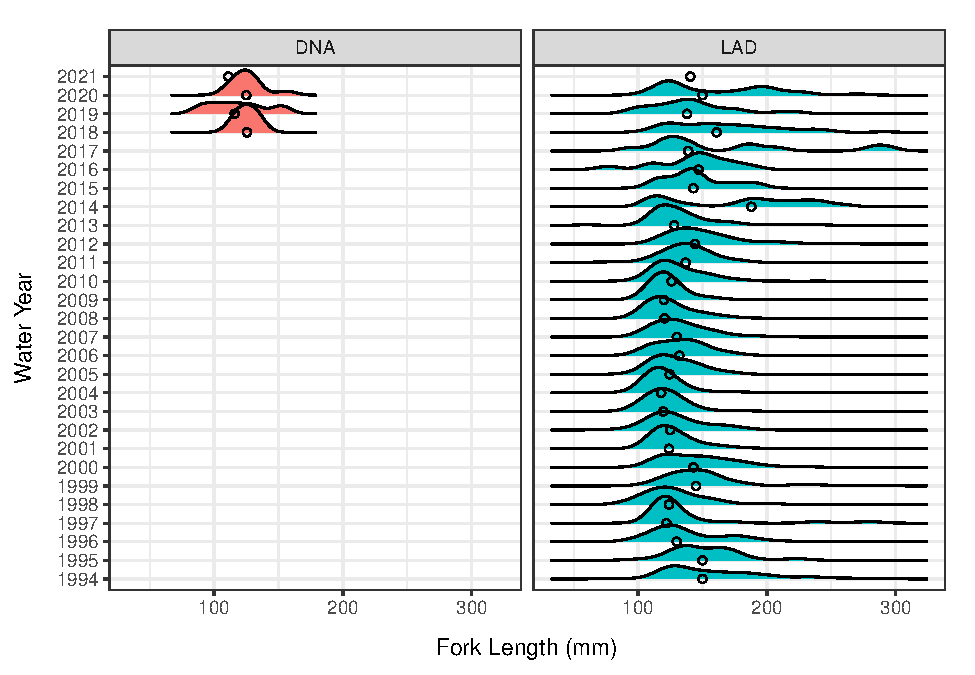
\includegraphics{_main_files/figure-latex/salvage_fl-fig-1.pdf}
\caption{(\#fig:salvage\_fl-fig)Fork Lengths of Genetic and LAD Winter Run Chinook Salmon Juveniles at Salvage. Points indicate median fork length.}
\end{figure}

\begin{figure}
\centering
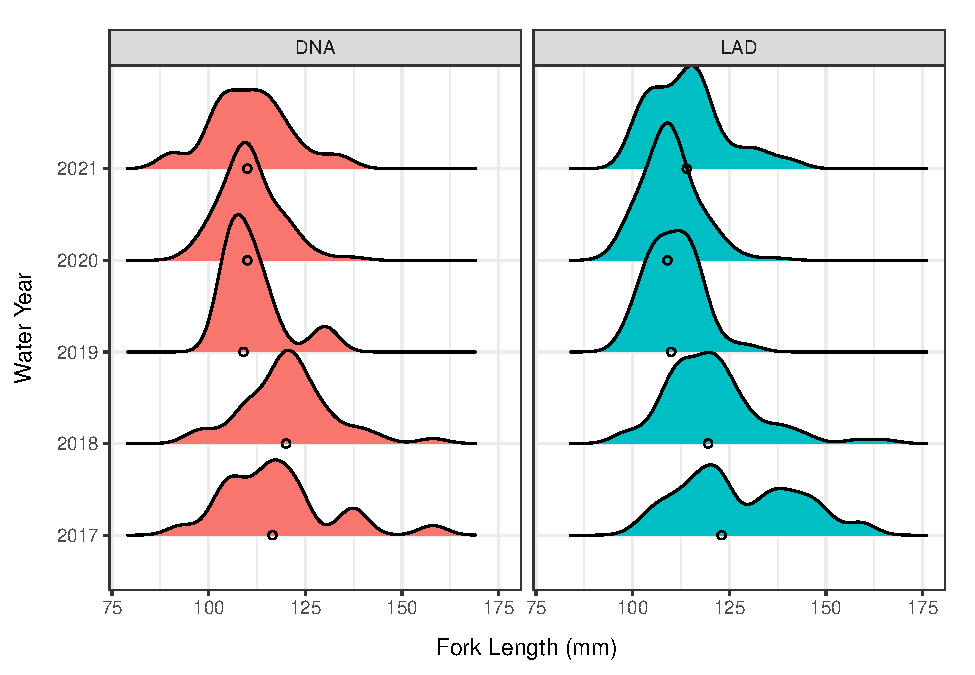
\includegraphics{_main_files/figure-latex/chipps_fl-fig-1.pdf}
\caption{(\#fig:chipps\_fl-fig)Fork Lengths of Genetic and LAD Winter Run Chinook Salmon Juveniles at Chipps Trawl. Points indicate median fork length.}
\end{figure}

\hypertarget{loss}{%
\subsection{Loss}\label{loss}}

Winter-run Current and Historic Cumulative Salvage (Line plots)

Current + Historic Percent of JPE

Monitoring Sources for abundance, growth/size, migration timing/duration

\begin{itemize}
\tightlist
\item
  Sac Trawl
\item
  Tisdale Weir
\item
  Knights Landing
\item
  GCID
\item
  DJFMP
\item
  Yolo Bypass
\item
  Chipps Island Trawl (Exit)
\item
  Genetic (Chipps, SWP/CVP, Knights Landing, Yolo Bypass)
\end{itemize}

\begin{enumerate}
\def\labelenumi{\arabic{enumi}.}
\item
  Abundance (Count) (IEP Monitoring)
\item
  Condition (IEP Monitoring)
\end{enumerate}

\begin{itemize}
\tightlist
\item
  FL
\end{itemize}

\begin{enumerate}
\def\labelenumi{\arabic{enumi}.}
\setcounter{enumi}{2}
\tightlist
\item
  Migration Timing (IEP Monitoring)
\end{enumerate}

\begin{itemize}
\tightlist
\item
  SacPAS style plots of historical and current year?
\end{itemize}

\emph{Chipps Trawl Timing}

\emph{Sac Trawl Timing}

\emph{Sac Beach Seine Timing}

\begin{enumerate}
\def\labelenumi{\arabic{enumi}.}
\setcounter{enumi}{3}
\tightlist
\item
  Migration Duration
\end{enumerate}

\begin{itemize}
\tightlist
\item
  Calfish Track/ERDDAP
\end{itemize}

\begin{enumerate}
\def\labelenumi{\arabic{enumi}.}
\setcounter{enumi}{4}
\item
  Migration Routing
\item
  Survival
\end{enumerate}

\begin{itemize}
\tightlist
\item
  Hatchery real-time: Calfish Track/ERDDAP
\item
  Natural Origin Smolt survival (O Farell et al.~2018)
\item
  Hatchery Origin Smolt survival
\item
  Modeled: ** Juvenile: STARS ** Fish Model
\item
  Survival to Delta: Production (Hatchery JPE, Modeled JPE)
\end{itemize}

\hypertarget{abbreviations}{%
\chapter{Abbreviations}\label{abbreviations}}

CM = Conceptual Model
WRCS = Winter Run Chinook Salmon

\hypertarget{useful-info}{%
\chapter{Useful info}\label{useful-info}}

\hypertarget{parts}{%
\section{Parts}\label{parts}}

You can add parts to organize one or more book chapters together. Parts can be inserted at the top of an .Rmd file, before the first-level chapter heading in that same file.

Add a numbered part: \texttt{\#\ (PART)\ Act\ one\ \{-\}} (followed by \texttt{\#\ A\ chapter})

Add an unnumbered part: \texttt{\#\ (PART\textbackslash{}*)\ Act\ one\ \{-\}} (followed by \texttt{\#\ A\ chapter})

Add an appendix as a special kind of un-numbered part: \texttt{\#\ (APPENDIX)\ Other\ stuff\ \{-\}} (followed by \texttt{\#\ A\ chapter}). Chapters in an appendix are prepended with letters instead of numbers.

\hypertarget{footnotes-and-citations}{%
\section{Footnotes and citations}\label{footnotes-and-citations}}

\hypertarget{footnotes}{%
\subsection{Footnotes}\label{footnotes}}

Footnotes are put inside the square brackets after a caret \texttt{\^{}{[}{]}}. Like this one \footnote{This is a footnote.}.

\hypertarget{citations}{%
\subsection{Citations}\label{citations}}

Reference items in your bibliography file(s) using \texttt{@key}.

For example, we are using the \textbf{bookdown} package \citep{R-bookdown} (check out the last code chunk in index.Rmd to see how this citation key was added) in this sample book, which was built on top of R Markdown and \textbf{knitr} \citep{xie2015} (this citation was added manually in an external file book.bib).
Note that the \texttt{.bib} files need to be listed in the index.Rmd with the YAML \texttt{bibliography} key.

The RStudio Visual Markdown Editor can also make it easier to insert citations: \url{https://rstudio.github.io/visual-markdown-editing/\#/citations}

\hypertarget{blocks}{%
\section{Blocks}\label{blocks}}

\hypertarget{equations}{%
\subsection{Equations}\label{equations}}

Here is an equation.

\begin{equation} 
  f\left(k\right) = \binom{n}{k} p^k\left(1-p\right)^{n-k}
  \label{eq:binom}
\end{equation}

You may refer to using \texttt{\textbackslash{}@ref(eq:binom)}, like see Equation \eqref{eq:binom}.

\hypertarget{theorems-and-proofs}{%
\subsection{Theorems and proofs}\label{theorems-and-proofs}}

Labeled theorems can be referenced in text using \texttt{\textbackslash{}@ref(thm:tri)}, for example, check out this smart theorem \ref{thm:tri}.

\begin{theorem}
\protect\hypertarget{thm:tri}{}\label{thm:tri}For a right triangle, if \(c\) denotes the \emph{length} of the hypotenuse
and \(a\) and \(b\) denote the lengths of the \textbf{other} two sides, we have
\[a^2 + b^2 = c^2\]
\end{theorem}

Read more here \url{https://bookdown.org/yihui/bookdown/markdown-extensions-by-bookdown.html}.

\hypertarget{callout-blocks}{%
\subsection{Callout blocks}\label{callout-blocks}}

The R Markdown Cookbook provides more help on how to use custom blocks to design your own callouts: \url{https://bookdown.org/yihui/rmarkdown-cookbook/custom-blocks.html}

\hypertarget{cross}{%
\section{Cross-references}\label{cross}}

Cross-references make it easier for your readers to find and link to elements in your book.

\hypertarget{chapters-and-sub-chapters}{%
\subsection{Chapters and sub-chapters}\label{chapters-and-sub-chapters}}

There are two steps to cross-reference any heading:

\begin{enumerate}
\def\labelenumi{\arabic{enumi}.}
\tightlist
\item
  Label the heading: \texttt{\#\ Hello\ world\ \{\#nice-label\}}.

  \begin{itemize}
  \tightlist
  \item
    Leave the label off if you like the automated heading generated based on your heading title: for example, \texttt{\#\ Hello\ world} = \texttt{\#\ Hello\ world\ \{\#hello-world\}}.
  \item
    To label an un-numbered heading, use: \texttt{\#\ Hello\ world\ \{-\#nice-label\}} or \texttt{\{\#\ Hello\ world\ .unnumbered\}}.
  \end{itemize}
\item
  Next, reference the labeled heading anywhere in the text using \texttt{\textbackslash{}@ref(nice-label)}; for example, please see Chapter \ref{cross}.

  \begin{itemize}
  \tightlist
  \item
    If you prefer text as the link instead of a numbered reference use: \protect\hyperlink{cross}{any text you want can go here}.
  \end{itemize}
\end{enumerate}

\hypertarget{captioned-figures-and-tables}{%
\subsection{Captioned figures and tables}\label{captioned-figures-and-tables}}

Figures and tables \emph{with captions} can also be cross-referenced from elsewhere in your book using \texttt{\textbackslash{}@ref(fig:chunk-label)} and \texttt{\textbackslash{}@ref(tab:chunk-label)}, respectively.

See Figure \ref{fig:nice-fig}.

\begin{figure}

{\centering 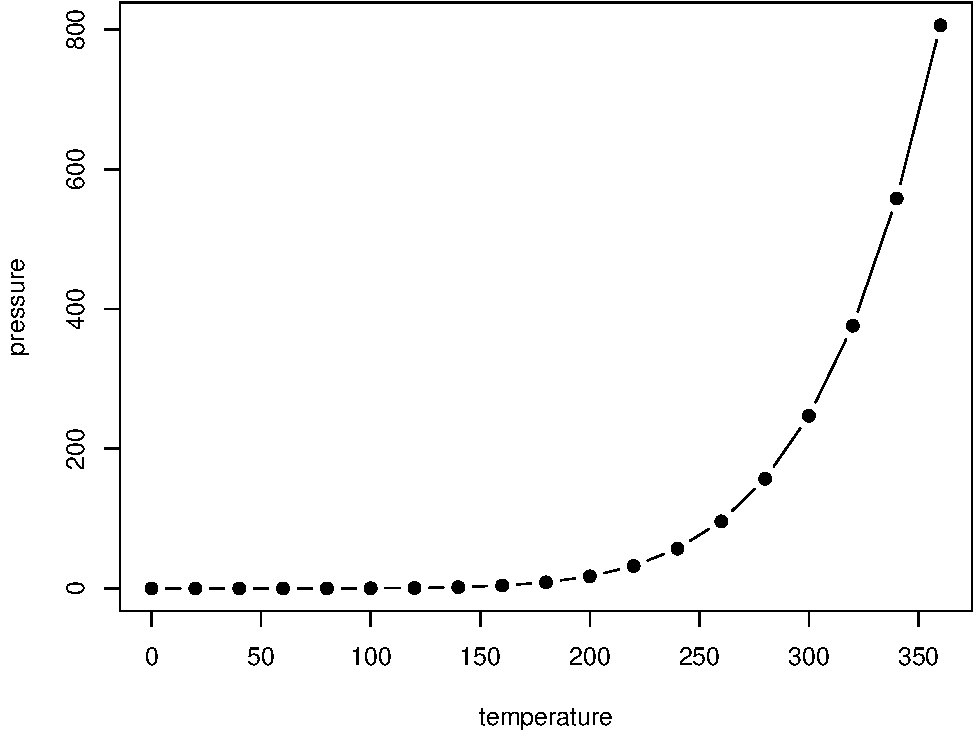
\includegraphics[width=0.8\linewidth]{_main_files/figure-latex/nice-fig-1} 

}

\caption{Here is a nice figure!}\label{fig:nice-fig}
\end{figure}

Don't miss Table \ref{tab:nice-tab}.

\begin{table}

\caption{\label{tab:nice-tab}Here is a nice table!}
\centering
\begin{tabular}[t]{rr}
\toprule
temperature & pressure\\
\midrule
0 & 0.0002\\
20 & 0.0012\\
40 & 0.0060\\
60 & 0.0300\\
80 & 0.0900\\
\addlinespace
100 & 0.2700\\
120 & 0.7500\\
140 & 1.8500\\
160 & 4.2000\\
180 & 8.8000\\
\bottomrule
\end{tabular}
\end{table}

\hypertarget{sharing-your-book}{%
\section{Sharing your book}\label{sharing-your-book}}

\hypertarget{publishing}{%
\subsection{Publishing}\label{publishing}}

HTML books can be published online, see: \url{https://bookdown.org/yihui/bookdown/publishing.html}

\hypertarget{pages}{%
\subsection{404 pages}\label{pages}}

By default, users will be directed to a 404 page if they try to access a webpage that cannot be found. If you'd like to customize your 404 page instead of using the default, you may add either a \texttt{\_404.Rmd} or \texttt{\_404.md} file to your project root and use code and/or Markdown syntax.

\hypertarget{metadata-for-sharing}{%
\subsection{Metadata for sharing}\label{metadata-for-sharing}}

Bookdown HTML books will provide HTML metadata for social sharing on platforms like Twitter, Facebook, and LinkedIn, using information you provide in the \texttt{index.Rmd} YAML. To setup, set the \texttt{url} for your book and the path to your \texttt{cover-image} file. Your book's \texttt{title} and \texttt{description} are also used.

This \texttt{gitbook} uses the same social sharing data across all chapters in your book- all links shared will look the same.

Specify your book's source repository on GitHub using the \texttt{edit} key under the configuration options in the \texttt{\_output.yml} file, which allows users to suggest an edit by linking to a chapter's source file.

Read more about the features of this output format here:

\url{https://pkgs.rstudio.com/bookdown/reference/gitbook.html}

Or use:

\hypertarget{render-book}{%
\section{Render book}\label{render-book}}

You can render the HTML version of this example book without changing anything:

\begin{enumerate}
\def\labelenumi{\arabic{enumi}.}
\item
  Find the \textbf{Build} pane in the RStudio IDE, and
\item
  Click on \textbf{Build Book}, then select your output format, or select ``All formats'' if you'd like to use multiple formats from the same book source files.
\end{enumerate}

Or build the book from the R console:

To render this example to PDF as a \texttt{bookdown::pdf\_book}, you'll need to install XeLaTeX. You are recommended to install TinyTeX (which includes XeLaTeX): \url{https://yihui.org/tinytex/}.

\hypertarget{preview-book}{%
\section{Preview book}\label{preview-book}}

As you work, you may start a local server to live preview this HTML book. This preview will update as you edit the book when you save individual .Rmd files. You can start the server in a work session by using the RStudio add-in ``Preview book'', or from the R console:

\hypertarget{footnotes-and-citations-1}{%
\section{Footnotes and citations}\label{footnotes-and-citations-1}}

\hypertarget{footnotes-1}{%
\subsection{Footnotes}\label{footnotes-1}}

Footnotes are put inside the square brackets after a caret \texttt{\^{}{[}{]}}. Like this one \footnote{This is a footnote.}.

\hypertarget{citations-1}{%
\subsection{Citations}\label{citations-1}}

\begin{itemize}
\tightlist
\item
  \url{https://www.anchorqea.com/news/brood-year-2019-winter-run-chinook-salmon-operations-and-monitoring-assessment/}
\end{itemize}

Reference items in your bibliography file(s) using \texttt{@key}.

For example, we are using the \textbf{bookdown} package \citep{R-bookdown} (check out the last code chunk in index.Rmd to see how this citation key was added) in this sample book, which was built on top of R Markdown and \textbf{knitr} \citep{xie2015} (this citation was added manually in an external file book.bib). Note that the \texttt{.bib} files need to be listed in the index.Rmd with the YAML \texttt{bibliography} key.

The RStudio Visual Markdown Editor can also make it easier to insert citations: \url{https://rstudio.github.io/visual-markdown-editing/\#/citations}

  \bibliography{book.bib,packages.bib}

\end{document}
